\documentclass[a4paper,12pt]{article}

% Packages
\usepackage[utf8]{inputenc} % For UTF-8 encoding
\usepackage[hungarian]{babel} % Hungarian language support
\usepackage{amsmath, amssymb} % Math symbols and environments
\usepackage{geometry} % Page geometry
\usepackage{titlesec} % Section formatting
\usepackage{enumitem} % Custom lists
\usepackage{hyperref} % Hyperlinks
\usepackage{fancyhdr} % Header and footer customization
\usepackage{graphicx} % Include graphics
\usepackage{multirow}
\usepackage{tikz}
\usepackage{pgfplots}
\usepgfplotslibrary{statistics}


% Page settings
\geometry{margin=1in}

% Title and author
\title{\textbf{Biostatisztika Záróvizsga Tételek}}
\author{Név: \textit{[Pinczés Dániel]}}
\date{\today}

% Header and footer
\pagestyle{fancy}
\fancyhf{}
\lhead{Záróvizsga Tételek}
\rhead{\thepage}

% Section formatting
\titleformat{\section}[block]{\bfseries\Large}{Tétel \thesection}{1em}{}
\titleformat{\subsection}[block]{\bfseries\large}{\thesubsection}{1em}{}

\begin{document}

% Title Page
    \maketitle
    \thispagestyle{empty}
    \newpage

% Table of Contents
    \tableofcontents
    \newpage

% Example Sections for Topics


    \section{A biostatisztika áttekintése: kérdésfeltevések és alapproblémák}

    \textbf{Tétel}:

    Tipikus problémák a biostatisztikában, a matematikailag megalapozott módszerek
    szükségessége az orvosbiológiai kutatások támogatásában. A humán empirikus orvosi
    kutatások módszerei, kísérlet és megfigyelés. A confounding fogalma. Védekezési
    lehetőségek a confounding ellen.

    \subsection{Tipikus problémák a biostatisztikában, a matematikailag megalapozott módszerek
    szükségessége az orvosbiológiai kutatások támogatásában.}
    Itt található az első tételhez tartozó első alcím részletezése.

    A biostatisztika az orvosi és biológiai kutatásokban felmerülő statisztikai kérdésekkel foglalkozik. Az "Az orvosi megismerés módszertana" című könyv számos példát hoz olyan kérdésekre, amelyek tipikusan előfordulnak az orvosi kutatásokban, és amelyek megválaszolásához statisztikai módszerekre van szükség. Ezek a kérdések általában ok-okozati összefüggések feltárására irányulnak.

    \begin{itemize}
        \item Környezeti tényezők és egészségügyi hatások

        "Okoz-e mentális betegséget a légszennyezettség?" (Forrás: 2. fejezet, 15. oldal) Ez a kérdés rávilágít arra, hogy a biostatisztikában gyakran vizsgálunk olyan problémákat, ahol egy környezeti tényező (jelen esetben a légszennyezettség) potenciális egészségügyi hatását szeretnénk felmérni.

        \item Technológiai fejlődés és egészségügyi kockázatok

        "A mobiltelefon-használat okoz-e agydaganatot?" (Forrás: 2. fejezet, 15. oldal) Ez a példa azt mutatja, hogy a biostatisztika fontos szerepet játszik az új technológiák potenciális egészségügyi kockázatainak értékelésében.

        \item Életmódbeli tényezők és betegségek kapcsolata

        "A vöröshús-fogyasztás növeli-e a vastagbélrák kockázatát?" (Forrás: 2. fejezet, 15. oldal) Ez a kérdés rámutat arra, hogy a biostatisztika gyakran foglalkozik olyan problémákkal, amelyek az életmód és a betegségek közötti összefüggéseket vizsgálják.

        \item Orvosi beavatkozások hosszú távú hatásai

        "A császármetszéssel születés növeli-e az 1-es típusú cukorbetegség kockázatát?" (Forrás: 2. fejezet, 15. oldal) Ez a példa azt illusztrálja, hogy a biostatisztika fontos szerepet játszik az orvosi beavatkozások hosszú távú következményeinek értékelésében.


        \item Gyógyszerek hatékonyságának vizsgálata

        "Egy új vérnyomáscsökkentő gyógyszer tényleg csökkenti-e a vérnyomást?" (Forrás: 2. fejezet, 15-16. oldal) Ez a kérdés rávilágít arra, hogy a biostatisztika kulcsfontosságú a gyógyszerek hatékonyságának és biztonságosságának értékelésében.

    \end{itemize}

    Az "Az orvosi megismerés módszertana" című könyv hangsúlyozza, hogy a matematikailag megalapozott módszerek elengedhetetlenek az orvosbiológiai kutatások támogatásában. Ennek több oka is van:

    \begin{itemize}

        \item Az empirikus megfigyelések önmagukban félrevezetőek lehetnek

        A könyv rámutat, hogy pusztán a megfigyelésekre hagyatkozva téves következtetésekre juthatunk. Erre kiváló példa az érvágás esete, amelyet a könyv részletesen tárgyal. Az érvágást évszázadokon át alkalmazták különböző betegségek gyógyítására, anélkül, hogy bárki empirikusan megvizsgálta volna annak tényleges hatásosságát. (Forrás: 1. fejezet, 8-10. oldal)

        \item A véletlen ingadozás hatásának kezelése:

        A könyv kifejti, hogy az orvosi kutatásokban mindig jelen van a véletlen ingadozás. Ez azt jelenti, hogy még akkor is kaphatunk eltérő eredményeket, ha valójában nincs valódi különbség vagy hatás. A matematikai módszerek segítenek abban, hogy megkülönböztessük a valódi hatásokat a véletlen ingadozásoktól. (Forrás: 5. fejezet, 47-48. oldal)

        \item Ok-okozati összefüggések feltárása

        A könyv hangsúlyozza, hogy az ok-okozati összefüggések feltárása komplex feladat. Nem elég csupán azt megállapítani, hogy két jelenség együtt jár, azt is ki kell mutatni, hogy az egyik okozza a másikat. Ehhez szükség van olyan matematikai módszerekre, amelyek képesek kezelni a zavaró tényezőket (confoundereket) és más komplex összefüggéseket. (Forrás: 2. fejezet, 16-17. oldal)

        \item A mintavételi hiba kezelése

        A könyv rámutat, hogy a kutatások során általában csak egy mintát tudunk vizsgálni, nem a teljes populációt. A matematikai módszerek segítenek abban, hogy a mintából nyert eredményeket megfelelően tudjuk általánosítani a teljes populációra. (Forrás: 5. fejezet, 64-65. oldal)

        \item A kutatások tervezése

        A matematikailag megalapozott módszerek nem csak az adatok elemzésében, hanem már a kutatások tervezésében is kulcsfontosságúak. A könyv részletesen tárgyalja, hogyan lehet meghatározni a szükséges mintaméretet, vagy hogyan lehet randomizálni a résztvevőket egy klinikai vizsgálatban. (Forrás: 5. fejezet, 68-71. oldal)

        \item A bizonytalanság számszerűsítése

        A könyv kiemeli, hogy a matematikai módszerek lehetővé teszik a bizonytalanság számszerűsítését. Ez segít abban, hogy ne csak azt tudjuk meg, mi a legjobb becslésünk egy hatás nagyságára, hanem azt is, mennyire lehetünk biztosak ebben a becslésben. (Forrás: 5. fejezet, 53-55. oldal)

    \end{itemize}

    A könyv konkrét példaként említi James Lind skorbut elleni kísérletét és Pierre-Charles-Alexandre Louis érvágással kapcsolatos vizsgálatát, amelyek a szisztematikus, empirikus vizsgálatok fontosságát demonstrálják. (Forrás: 1. fejezet, 10-11. oldal)

    Saját kiegészítés: Fontos megjegyezni, hogy a matematikailag megalapozott módszerek nem helyettesítik, hanem kiegészítik az orvosi szakértelmet. A statisztikai eredmények értelmezéséhez és a klinikai gyakorlatba való átültetéséhez továbbra is szükség van az orvosok szakértelmére és tapasztalatára. A matematikai módszerek inkább eszközök, amelyek segítik az orvosokat a jobb döntéshozatalban és a tudományos bizonyítékok értékelésében.

    \subsection{A humán empirikus orvosi kutatások módszerei, kísérlet és megfigyelés}

    Az orvosi kutatásokban két fő módszert különböztetünk meg az empirikus vizsgálatok során: a kísérletet és a megfigyelést. A könyv részletesen tárgyalja mindkét módszert, kiemelve azok előnyeit és hátrányait.

    \subsubsection{Kísérlet}

    A kísérlet során a kutatók aktívan befolyásolják az expozíciót, vagyis azt a tényezőt, amelynek a hatását vizsgálni szeretnék.

    \begin{itemize}

        \item \textbf{Jellemzői}: A kutatók döntik el, ki kerül a kezelt és ki a kontroll csoportba. Lehetővé teszi a randomizációt, ami a leghatékonyabb módszer a confounding ellen. Általában kisebb mintamérettel dolgozik, mint a megfigyeléses vizsgálatok. Az utánkövetési idő gyakran korlátozott.

        \item \textbf{Példa}: James Lind skorbut elleni kísérlete, ahol a tengerészeket különböző csoportokba osztotta, és eltérő kezeléseket alkalmazott. (Forrás: 1. fejezet, 11. oldal)

        \item \textbf{Előnyök}: Lehetővé teszi az ok-okozati összefüggések közvetlen vizsgálatát.
        A randomizáció révén kiküszöböli a confounding hatását.

        \item \textbf{Hátrányok}: Etikai korlátok (pl. nem lehet szándékosan káros expozíciónak kitenni az alanyokat).
        Költséges és időigényes lehet.
        A résztvevők összetétele gyakran eltér a teljes populációétól. (Forrás: 3. fejezet, 27-30. oldal)

    \end{itemize}

    \subsubsection{Megfigyelés}

    A megfigyeléses vizsgálatok során a kutatók nem befolyásolják az expozíciót, csak megfigyelik és rögzítik az eseményeket.

    \begin{itemize}

        \item \textbf{Jellemzői}: A kutatók nem avatkoznak be az expozíció kiosztásába.
        Általában nagyobb mintamérettel dolgozik.
        Hosszabb utánkövetési idő lehetséges.
        A vizsgált populáció jobban reprezentálja a teljes populációt.
        Példa: A légszennyezettség és a mentális betegségek kapcsolatának vizsgálata, ahol a kutatók nem befolyásolják, ki él szennyezett területen. (Forrás: 2. fejezet, 15. oldal)

        \item  \textbf{Előnyök}: Etikailag kevésbé problémás.
        Nagyobb mintaméret és hosszabb utánkövetési idő lehetséges.
        Jobban reprezentálja a valós életbeli körülményeket.

        \item \textbf{Hátrányok}: Nehezebb az ok-okozati összefüggések megállapítása.
        A confounding problémája jelentősebb.
    \end{itemize}


    (Forrás: 3. fejezet, 28-30. oldal)

    A könyv hangsúlyozza, hogy mindkét módszernek megvan a maga helye az orvosi kutatásokban. A kísérletek erőssége, hogy jobban kontrollálhatók és alkalmasabbak ok-okozati összefüggések feltárására. A megfigyeléses vizsgálatok viszont jobban tükrözik a valós életbeli körülményeket, és olyan helyzetekben is alkalmazhatók, ahol a kísérletek etikailag vagy gyakorlatilag nem kivitelezhetők.

    A könyv egy érdekes példát hoz az ejtőernyők hatékonyságának vizsgálatára, ami jól szemlélteti a kétféle módszer közötti különbséget és azok korlátait. (Forrás: 3. fejezet, 30-31. oldal)

    Saját kiegészítés: Fontos megjegyezni, hogy a modern orvosi kutatásokban gyakran kombinálják a kétféle megközelítést. Például egy megfigyeléses vizsgálat eredményei alapján hipotéziseket állítanak fel, amelyeket aztán klinikai kísérletekben tesztelnek. Vagy fordítva, egy klinikai kísérlet eredményeit későbbi megfigyeléses vizsgálatokkal validálják a való életben. Ez a kombinált megközelítés segít kihasználni mindkét módszer előnyeit, miközben minimalizálja azok hátrányait.

    \subsection{A confounding fogalma}

    A confounding (zavaró tényező) az orvosi kutatások egyik legfontosabb és leggyakoribb problémája. A könyv részletesen tárgyalja ezt a jelenséget, annak jelentőségét és következményeit.

    \textbf{Definíció}: A confounding olyan változó, amely egyszerre összefügg az expozícióval (a vizsgált tényezővel) és a végponttal (a vizsgált kimenetellel), ezáltal torzíthatja az eredményeket és hamis összefüggéseket sugallhat. (Forrás: 2. fejezet, 17-18. oldal)

    Példa a könyvből: A könyv egy szemléletes példát hoz a légszennyezettség és a mentális betegségek kapcsolatának vizsgálatára. Ebben az esetben a szocioökonómiai helyzet lehet confounder, mert:

    \begin{itemize}

        \item Összefügg az expozícióval

        A rosszabb szocioökonómiai helyzetű emberek gyakrabban élnek szennyezettebb területeken.

        \item Összefügg a végponttal

        A rosszabb szocioökonómiai helyzetű emberek körében gyakoribbak a mentális betegségek.

    \end{itemize}

    Így, ha csak a légszennyezettség és a mentális betegségek előfordulása közötti kapcsolatot vizsgáljuk, tévesen azt gondolhatjuk, hogy a légszennyezettség okozza a mentális betegségeket, holott valójában a szocioökonómiai helyzet állhat mindkettő hátterében. (Forrás: 2. fejezet, 17-20. oldal)

    \textbf{A confounding hatása}

    \begin{itemize}

        \item Hamis összefüggéseket mutathat ki
        Olyan kapcsolatot sugallhat két változó között, amely valójában nem létezik.


        \item Elfedheti a valódi összefüggéseket
        Elképzelhető, hogy van valódi kapcsolat két változó között, de a confounder miatt ezt nem tudjuk kimutatni.


        \item Torzíthatja a hatás nagyságát
        Még ha van is valódi kapcsolat, a confounder miatt túl- vagy alulbecsülhetjük annak mértékét.
    \end{itemize}

    A confounding felismerésének nehézségei: A könyv hangsúlyozza, hogy a confounding felismerése nem mindig egyszerű. Néha nyilvánvaló lehet (mint a fenti példában), de gyakran rejtett és nehezen azonosítható. Ráadásul egy vizsgálatban több confounder is jelen lehet egyidejűleg, tovább bonyolítva a helyzetet. (Forrás: 2. fejezet, 19-20. oldal)

    A confounding jelentősége: A könyv kiemeli, hogy a confounding figyelmen kívül hagyása súlyos következményekkel járhat. Téves következtetésekre juthatunk az ok-okozati összefüggésekről, ami helytelen klinikai döntésekhez vagy közegészségügyi intézkedésekhez vezethet. (Forrás: 2. fejezet, 20-23. oldal)

    Történeti példa: A könyv egy érdekes történeti példát is hoz a confounding problémájára. A 18. században Daniel Bernoulli azt vizsgálta, hogy miért magasabb a halálozási ráta a városokban, mint vidéken. Első ránézésre úgy tűnt, hogy a városi élet káros az egészségre. Azonban Bernoulli rájött, hogy az életkor egy confounder ebben az esetben: a városokba több fiatal költözött munkát keresni, és mivel a fiatalok általában egészségesebbek, ez torzította az összehasonlítást. (Forrás: 2. fejezet, 21-22. oldal)

    Saját kiegészítés: Fontos megjegyezni, hogy a confounding problémája nem csak az orvosi kutatásokban, hanem minden olyan területen jelentkezhet, ahol ok-okozati összefüggéseket próbálunk feltárni. Például a társadalomtudományokban, a pszichológiában vagy akár a gazdasági elemzésekben is kulcsfontosságú a zavaró tényezők azonosítása és kezelése. Az orvosi kutatásokban azért különösen kritikus ez a kérdés, mert a téves következtetések közvetlenül befolyásolhatják az emberek egészségét és életét.

    \subsection{Védekezési lehetőségek a confounding ellen}

    A könyv több módszert is ismertet, amelyekkel védekezhetünk a confounding hatása ellen. Ezek a módszerek segítenek abban, hogy pontosabb és megbízhatóbb következtetéseket vonhassunk le az orvosi kutatásokban.

    \subsubsection{Randomizáció}

    Ez a módszer kísérletes vizsgálatokban alkalmazható.

    \begin{itemize}
        \item \textbf{Lényege}
        A résztvevőket véletlenszerűen osztjuk be a különböző csoportokba (pl. kezelt és kontroll csoport).

        \item \textbf{Előnye}
        Ez a leghatékonyabb módszer, mert minden confoundert kiszűr, még azokat is, amelyekre nem gondoltunk.

        \item \textbf{Történeti példa}:
        James Burns Amberson 1931-es kísérlete, ahol pénzfeldobással döntötte el, hogy ki kapjon sanocrysin-t a TBC kezelésére.

        \item \textbf{Működési elv}:
        A randomizáció biztosítja, hogy a csoportok csak a vizsgált tényezőben (expozícióban) térjenek el egymástól, minden más szempontból hasonlóak legyenek.
        (Forrás: 3. fejezet, 26-27. oldal)

    \end{itemize}

    \subsubsection{Rétegzés}

    Ez a módszer megfigyeléses vizsgálatokban alkalmazható.

    \begin{itemize}
        \item \textbf{Lényege}: A confounding változó szerint rétegekre bontjuk a mintát, és rétegenként külön-külön végezzük el az elemzést.
        \item \textbf{Példa}: Ha az életkor a confounder, akkor külön vizsgáljuk az összefüggést a fiatalok, középkorúak és idősek csoportjában.
        \item \textbf{Előnye}: Egyszerű módszer, nem igényel bonyolult statisztikai eljárásokat.
        \item \textbf{Hátránya}: Ha sok confounder van, vagy folytonos változók (pl. életkor) esetén nehezen alkalmazható.
    \end{itemize}
    (Forrás: 4. fejezet, 33-35. oldal)

    \subsubsection{Standardizálás}

    Ez is megfigyeléses vizsgálatokban használatos módszer.

    \begin{itemize}
        \item \textbf{Lényege}: A confounding változó eloszlását egységesítjük a csoportok között, így téve összehasonlíthatóvá az eredményeket.
        \item \textbf{Példa}: A könyv részletesen tárgyalja a halálozási ráták standardizálását életkor szerint különböző országok összehasonlításakor.
        \item \textbf{Előnye}: Lehetővé teszi az összehasonlítást olyan esetekben is, amikor a csoportok összetétele nagyon eltérő.
        \item \textbf{Alkalmazás}: Gyakran használják epidemiológiai vizsgálatokban, például országok egészségügyi mutatóinak összehasonlításakor.
    \end{itemize}
    (Forrás: 4. fejezet, 35-43. oldal)

    \subsubsection{Többváltozós regressziós modellezés}

    A könyv említi, de részletesen nem tárgyalja ezt a módszert.

    \begin{itemize}
        \item \textbf{Lényege}: Statisztikai modelleket használunk, amelyek egyszerre több változó hatását tudják figyelembe venni.
        \item \textbf{Előnye}: Lehetővé teszi több confounder egyidejű kezelését.
        \item \textbf{Alkalmazás}: Széles körben használt módszer a modern orvosi kutatásokban.
    \end{itemize}

    (Forrás: 4. fejezet, 33. oldal)

    \subsubsection{Megfelelő kutatási terv}

    A könyv hangsúlyozza, hogy a confounding elleni védekezés már a kutatás tervezési fázisában elkezdődik.

    \begin{itemize}
        \item \textbf{Lényege}: Alapos előzetes tervezéssel azonosítjuk a potenciális confoundereket és beépítjük kezelésüket a kutatási tervbe.
        \item \textbf{Példa}: Adatgyűjtés során rögzítjük a releváns háttérváltozókat, amelyek később confounderként viselkedhetnek.
    \end{itemize}

    A könyv kiemeli, hogy a confounding kezelése kulcsfontosságú az orvosi kutatásokban, mert enélkül téves következtetésekre juthatunk az ok-okozati összefüggésekről. Ugyanakkor azt is hangsúlyozza, hogy a megfigyeléses vizsgálatokban soha nem lehetünk teljesen biztosak abban, hogy minden confoundert sikerült azonosítanunk és kezelnünk.

    Saját kiegészítés: Fontos megjegyezni, hogy a modern orvosi kutatásokban gyakran kombinálják ezeket a módszereket. Például egy megfigyeléses vizsgálatban alkalmazhatnak rétegzést és standardizálást is, majd az eredményeket többváltozós regressziós modellekkel ellenőrizhetik. Emellett az utóbbi években egyre nagyobb szerepet kapnak a fejlett statisztikai módszerek, mint például a propensity score matching vagy az instrumentális változók módszere, amelyek további lehetőségeket kínálnak a confounding kezelésére.


    \newpage


    \section{Az orvosi kutatások vizsgálati módszerei}

    \textbf{Tétel}:

    A vizsgálati módszerek csoportosítása. Megfigyeléses vizsgálatok: egyedi adatok alapuló
    vizsgálatok (kohorsz, eset-kontroll), aggregált adatokon alapuló (ecological) vizsgálatok,
    kontroll nélküli vizsgálatok. Kísérletes vizsgálatok jellemzői. Metaanalízisek fogalma, szerepe,
    fontossága.

    \subsection{A vizsgálati módszerek csoportosítása}

    Az "Az orvosi megismerés módszertana" című könyv alapján az orvosi kutatásokban alkalmazott vizsgálati módszereket alapvetően három fő csoportba sorolhatjuk:

    \textbf{Megfigyeléses vizsgálatok}
    \begin{itemize}
        \item A kutatók nem avatkoznak be az expozíció kiosztásába, csak megfigyelik és rögzítik az eseményeket.
        \item Ide tartoznak az egyedi és aggregált adatokon alapuló vizsgálatok, valamint a kontroll nélküli vizsgálatok.
    \end{itemize}

    \textbf{Kísérletes vizsgálatok}
    \begin{itemize}
        \item A kutatók aktívan befolyásolják az expozíciót.
        \item Lehetővé teszik a randomizációt és a kontrollált körülmények közötti vizsgálatot.
    \end{itemize}

    \textbf{Metaanalízisek}
    \begin{itemize}
        \item Több, azonos kérdést vizsgáló kutatás eredményeinek statisztikai összegzése.
        \item Nem új adatgyűjtésen, hanem meglévő kutatások szintézisén alapul.
    \end{itemize}

    A könyv hangsúlyozza, hogy mindegyik módszernek megvan a maga helye és szerepe az orvosi kutatásokban. A módszerek közötti választást befolyásoló fő tényezők:

    \begin{itemize}
        \item A kutatási kérdés jellege
        \item Etikai megfontolások
        \item Gyakorlati megvalósíthatóság
        \item Rendelkezésre álló erőforrások
    \end{itemize}

    (Forrás: 3. fejezet, 27-30. oldal)

    \subsection{Megfigyeléses vizsgálatok}

    A megfigyeléses vizsgálatok olyan kutatási módszerek, ahol a kutatók nem avatkoznak be az expozíció kiosztásába, hanem passzívan figyelik meg és rögzítik az eseményeket. A könyv több típusú megfigyeléses vizsgálatot is tárgyal:

    \subsubsection{Egyedi adatokon alapuló vizsgálatok}

    \begin{enumerate}[label=(\alph*)]

        \item Kohorsz vizsgálatok

        \begin{itemize}
            \item textbf{Definíció}: Egy populációt hosszabb időn át követnek, és figyelik, hogy kik betegszenek meg.

            \item \textbf{Jellemzők}: Prospektív jellegű (előre tekintő)
            Az expozíciótól haladnak a végpont felé
            Alkalmas ritka expozíciók vizsgálatára

            \item  \textbf{Előnyök}: Időbeli sorrend tisztázható, több végpont is vizsgálható

            \item \textbf{Hátrányok}: Hosszú idő, drága, nem alkalmas ritka betegségek vizsgálatára

            \item \textbf{Példa}: A Framingham Heart Study, amely 1948-ban kezdődött, és több ezer embert követett évtizedeken át, hogy azonosítsa a szív- és érrendszeri betegségek kockázati tényezőit. (Forrás: 4. fejezet, 34. oldal)
        \end{itemize}

        \item Eset-kontroll vizsgálatok
        \begin{itemize}

            \item \textbf{Definíció}: Beteg (eset) és nem beteg (kontroll) csoportokat hasonlítanak össze a múltbeli expozíciók tekintetében.

            \item \textbf{Jellemzők}: Retrospektív jellegű (visszatekintő). A végponttól haladnak az expozíció felé. Alkalmas ritka betegségek vizsgálatára.


            \item \textbf{Előnyök}: Gyors, olcsó, jó ritka betegségekre

            \item \textbf{Hátrányok}: Nehéz megfelelő kontrollcsoportot találni, emlékezeti torzítás lehetősége

            \item \textbf{Példa}: Richard Doll és Austin Bradford Hill dohányzás és tüdőrák kapcsolatát vizsgáló kutatása az 1950-es években. Tüdőrákos betegeket (esetek) hasonlítottak össze nem tüdőrákos emberekkel (kontrollok), és vizsgálták a dohányzási szokásaikat. (Forrás: 4. fejezet, 35. oldal)

        \end{itemize}
        (Forrás: 4. fejezet, 33-35. oldal)

    \end{enumerate}

    \subsubsection{Aggregált adatokon alapuló (ecological) vizsgálatok}

    \begin{itemize}

        \item  \textbf{Definíció}: Nem egyénekre, hanem csoportokra vonatkozó adatokat elemeznek.

        \item \textbf{Jellemzők}:
        Populáció szintű adatokat használnak
        Gyorsan és olcsón kivitelezhetők

        \item \textbf{Előnyök}: Nagy populációkat lehet vizsgálni, olcsó.

        \item \textbf{Hátrányok}: Ökológiai tévkövetkeztetés veszélye (amit csoportszinten látunk, nem feltétlenül igaz egyéni szinten)

        \item \textbf{Példa}: A könyv említi az országok közötti összehasonlításokat, például a halálozási ráták összehasonlítását különböző országokban. (Forrás: 4. fejezet, 38-41. oldal)


    \end{itemize}

    \subsubsection{Kontroll nélküli vizsgálatok}

    \begin{itemize}

        \item \textbf{Definíció}: Egyetlen csoport megfigyelése kontrollcsoport nélkül.

        \item \textbf{Jellemzők}:
        Általában egy beavatkozás előtti és utáni állapotot hasonlítanak össze

        \item \textbf{Előnyök}: Egyszerű, gyors

        \item \textbf{Hátrányok}: Nem lehet kiszűrni az időbeli trendek hatását, confounding problémája jelentős

        \item \textbf{Példa}
        A könyv nem ad konkrét példát erre a típusra, de megemlíti, hogy ezek általában egy beavatkozás előtti és utáni állapotot hasonlítanak össze.\textbf{Elméleti illusztráció}: Egy új gyógyszer hatásosságának vizsgálata magas vérnyomásban szenvedő betegeknél. A kutatók kiválasztanak egy csoport magas vérnyomású beteget, megmérik a vérnyomásukat, majd elkezdik adni nekik az új gyógyszert. Egy meghatározott idő után (pl. 3 hónap) újra megmérik a vérnyomásukat, és összehasonlítják a kezdeti értékekkel.

    \end{itemize}

    A könyv hangsúlyozza, hogy a megfigyeléses vizsgálatok fő előnye, hogy valós életbeli körülményeket tükröznek, és olyan helyzetekben is alkalmazhatók, ahol kísérletek etikailag vagy gyakorlatilag nem kivitelezhetők. Ugyanakkor a fő hátrányuk, hogy nehezebb az ok-okozati összefüggések megállapítása, és a confounding problémája jelentősebb.

    (Forrás: 4. fejezet, 33-43. oldal)

    Saját kiegészítés: Fontos megjegyezni, hogy a modern epidemiológiában egyre kifinomultabb statisztikai módszereket alkalmaznak a megfigyeléses vizsgálatok elemzésére, hogy minimalizálják a confounding és egyéb torzítások hatását. Ilyen módszerek például a propensity score matching vagy az instrumentális változók módszere. Ezek segíthetnek abban, hogy a megfigyeléses vizsgálatok eredményei megbízhatóbbak legyenek, bár természetesen nem helyettesíthetik teljesen a randomizált kísérleteket.

    \subsection{Kísérletes vizsgálatok jellemzői}

    \subsubsection{Definíció}
    Kísérletes vizsgálatokban a kutatók aktívan befolyásolják az expozíciót, vagyis azt a tényezőt, amelynek a hatását vizsgálni szeretnék.

    (Forrás: 3. fejezet, 27. oldal)

    \subsubsection{Fő jellemzők}

    \paragraph{Beavatkozás az expozícióba:}
    \begin{itemize}
        \item A kutatók döntik el, ki kerül a kezelt és ki a kontroll csoportba.
        \item Ez lehetővé teszi az ok-okozati összefüggések közvetlen vizsgálatát.
    \end{itemize}

    \paragraph{Randomizáció:}
    \begin{itemize}
        \item A résztvevőket véletlenszerűen osztják be a csoportokba.
        \item Ez a leghatékonyabb módszer a confounding kiküszöbölésére.
        \item Példa: James Burns Amberson 1931-es TBC-kísérlete, ahol pénzfeldobással döntötte el, ki kap kezelést.
    \end{itemize}

    (Forrás: 3. fejezet, 26. oldal)

    \paragraph{Kontrollcsoport használata:}
    \begin{itemize}
        \item Lehetővé teszi a kezelés hatásának összehasonlítását a kezelés nélküli állapottal.
        \item Gyakran placebo-kontrollt alkalmaznak.
    \end{itemize}

    \paragraph{Vakosítás:}
    \begin{itemize}
        \item Egyszeresen vak: a résztvevők nem tudják, melyik csoportba kerültek.
        \item Kettősen vak: sem a résztvevők, sem a kutatók nem tudják, ki melyik csoportban van.
        \item Célja a torzítások csökkentése.
    \end{itemize}

    \subsubsection{Előnyök és hátrányok}

    \paragraph{Előnyök:}
    \begin{itemize}
        \item Lehetővé teszi az ok-okozati összefüggések közvetlen vizsgálatát.
        \item A randomizáció révén kiküszöböli a confounding hatását.
        \item Jól kontrollált körülmények között vizsgálhatók a hatások.
    \end{itemize}

    \paragraph{Hátrányok:}
    \begin{itemize}
        \item Etikai korlátok (pl. nem lehet szándékosan káros expozíciónak kitenni az alanyokat).
        \item Költséges és időigényes lehet.
        \item A résztvevők összetétele gyakran eltér a teljes populációétól (szelekciós torzítás).
        \item Általában kisebb mintamérettel dolgozik, mint a megfigyeléses vizsgálatok.
        \item Az utánkövetési idő gyakran korlátozott.
    \end{itemize}

    (Forrás: 3. fejezet, 27-31. oldal)

    \subsubsection{Alkalmazási területek}
    \begin{itemize}
        \item Gyógyszervizsgálatok
        \item Új terápiás eljárások tesztelése
        \item Prevenciós stratégiák hatékonyságának vizsgálata
    \end{itemize}

    \subsubsection{Etikai megfontolások}
    \begin{itemize}
        \item Minden kísérletes vizsgálathoz etikai bizottsági engedély szükséges.
        \item A résztvevők tájékozott beleegyezése elengedhetetlen.
        \item A potenciális kockázatokat és előnyöket gondosan mérlegelni kell.
    \end{itemize}

    \subsubsection{Példák}
    \begin{itemize}
        \item James Lind skorbut elleni kísérlete (1747)
        \item Az ISIS-2 vizsgálat, amely az aszpirin és sztreptokináznak nevezett vérrögoldó hatását vizsgálta infarktusban (1988)
    \end{itemize}

    (Forrás: 3. fejezet, 27-31. oldal, 6. fejezet, 88-89. oldal)

    \subsection{Metaanalízisek fogalma, szerepe, fontossága}

    \subsubsection{Fogalom}
    A metaanalízis több, azonos kérdést vizsgáló kutatás eredményeinek statisztikai összegzése. Ez egy szisztematikus módszer, amely lehetővé teszi, hogy különböző vizsgálatok eredményeit együttesen értékeljük és vonjunk le következtetéseket.

    (Forrás: 3. fejezet, 29. oldal)

    \subsubsection{Szerepe}

    \paragraph{Bizonyítékok szintézise:}
    A metaanalízis lehetővé teszi, hogy egy adott kutatási kérdésről átfogóbb képet kapjunk, mint amit egyetlen vizsgálat eredményei alapján kaphatnánk.

    \paragraph{Statisztikai erő növelése:}
    Az egyes vizsgálatok eredményeinek összevonásával növelhető a statisztikai erő, ami különösen fontos lehet ritka események vagy kis hatások kimutatásánál.

    \paragraph{Ellentmondások feloldása:}
    Ha különböző vizsgálatok ellentmondó eredményeket mutatnak, a metaanalízis segíthet tisztázni az összképet.

    \paragraph{Új hipotézisek generálása:}
    Az összesített adatok elemzése során új összefüggések, hipotézisek merülhetnek fel.

    \subsubsection{Fontossága}

    \paragraph{Magasabb szintű bizonyíték:}
    A metaanalízisek az evidencia-alapú orvoslás hierarchiájában magasabb szinten állnak, mint az egyedi vizsgálatok. Ez azt jelenti, hogy erősebb bizonyítékot szolgáltatnak egy adott kérdésben.

    \paragraph{Klinikai döntéshozatal támogatása:}
    Az összesített eredmények segíthetnek az orvosoknak a legjobb kezelési módok kiválasztásában.

    \paragraph{Kutatási irányok meghatározása:}
    A metaanalízisek rámutathatnak olyan területekre, ahol további kutatásokra van szükség.

    \paragraph{Erőforrások hatékony felhasználása:}
    Ahelyett, hogy újabb és újabb hasonló vizsgálatokat végeznének, a kutatók a meglévő eredményeket szintetizálhatják, ami idő- és költséghatékony.

    \subsubsection{Korlátok és kihívások}
    A könyv megemlíti, hogy bár a metaanalízisek rendkívül hasznosak, vannak korlátaik is:

    \paragraph{Publikációs torzítás:}
    A negatív eredményű vizsgálatokat ritkábban publikálják, ami torzíthatja a metaanalízis eredményeit.

    \paragraph{Heterogenitás:}
    Az összevont vizsgálatok között lehetnek módszertani vagy populációs különbségek, amelyek megnehezítik az összehasonlítást.

    \paragraph{Minőségi kérdések:}
    A metaanalízis eredménye csak olyan jó lehet, mint az alapjául szolgáló vizsgálatok minősége.

    (Forrás: 3. fejezet, 29-30. oldal)

    \newpage


    \section{Deskriptív statisztika: kategoriális változó(k) vizsgálata}

    \paragraph{Tétel:} Analitikus módszerek kategoriális változó vizsgálatára: gyakorisági sor, gyakoriság, relatív
    gyakoriság, módusz. Grafikus módszer kategoriális változó vizsgálatára: oszlop- és
    kördiagram. Két kategoriális változó egyidejű vizsgálata, kereszttábla.

    \subsection{Analitikus módszerek kategoriális változó vizsgálatára}

    \subsubsection{Gyakorisági sor}
    A gyakorisági sor a kategoriális változó lehetséges kimeneteit (kategóriáit) tartalmazza, együtt azzal, hogy az adott kimenet hányszor fordult elő az adatbázisban.
    (Forrás: 19. oldal)

    \begin{description}
        \item[Példa:] Tekintsük egy kórház betegfelvételi osztályán egy nap alatt felvett betegek nemét:
        \begin{center}
            \begin{tabular}{|c|c|}
                \hline
                Nem   & Gyakoriság \\
                \hline
                Férfi & 45         \\
                Nő    & 55         \\
                \hline
            \end{tabular}
        \end{center}
        Ez a táblázat a nem változó gyakorisági sora.
    \end{description}

    \subsubsection{Gyakoriság}
    A gyakoriság az adott kategória előfordulásainak száma az adatbázisban. A statisztikában általában $f$-fel jelölik. Ha az $i$-edik kategória gyakoriságáról van szó, akkor $f_i$-vel jelölik.
    (Forrás: 19. oldal)

    \begin{description}
        \item[Példa:] A fenti példában $f_{\text{férfi}} = 45$ és $f_{\text{nő}} = 55$.
    \end{description}

    \subsubsection{Relatív gyakoriság}
    A relatív gyakoriság az abszolút gyakoriság osztva a mintanagysággal ($n$-nel). Azt mutatja meg, hogy egy kategóriába a megfigyelési egységek mekkora hányada esik. A relatív gyakoriságok összege mindig 1.
    (Forrás: 19-20. oldal)

    \begin{description}
        \item[Példa:] A fenti példában a relatív gyakoriságok:
        \begin{align*}
            \text{Férfi: } & \frac{45}{100} = 0,45 \text{ vagy } 45\% \\
            \text{Nő: } & \frac{55}{100} = 0,55 \text{ vagy } 55\%
        \end{align*}
    \end{description}

    \subsubsection{Módusz}
    A módusz a leggyakoribb kimenet, azaz az a kategória, amelyhez tartozó gyakoriság a legnagyobb az adatbázisban. Jelölése: Mo.
    (Forrás: 20. oldal)

    \begin{description}
        \item[Példa:] A fenti példában a módusz a "Nő" kategória, mivel ennek a legnagyobb a gyakorisága (55).
    \end{description}

    \subsubsection{Kiegészítések}

    \paragraph{Kumulált gyakoriság és kumulált relatív gyakoriság}
    Bár a könyv itt nem említi, de ordinális kategoriális változók esetén értelmezhető a kumulált gyakoriság ($f'$) és a kumulált relatív gyakoriság ($g'$) fogalma is. Ezek adott kategóriáig összegzik a gyakoriságokat, illetve relatív gyakoriságokat.

    \begin{description}
        \item[Példa:] Tekintsük egy fájdalomcsillapító hatékonyságának értékelését:
        \begin{center}
            \begin{tabular}{|c|c|c|c|}
                \hline
                Értékelés         & Gyakoriság & Kumulált gyakoriság & Kumulált relatív gyakoriság \\
                \hline
                Nem hatásos       & 10         & 10                  & 0,1                         \\
                Kissé hatásos     & 30         & 40                  & 0,4                         \\
                Közepesen hatásos & 40         & 80                  & 0,8                         \\
                Nagyon hatásos    & 20         & 100                 & 1,0                         \\
                \hline
            \end{tabular}
        \end{center}
    \end{description}

    \paragraph{Mintanagyság}
    A mintanagyságot általában $n$-nel jelölik, és ez a gyakoriságok összege: $\sum_{i=1}^n f_i = n$.
    (Forrás: 19. oldal)

    \begin{description}
        \item[Példa:] A betegfelvételi példában $n = 45 + 55 = 100$.
    \end{description}

    \paragraph{Megoszlás}
    A teljes relatív gyakorisági sort a statisztikusok gyakran a változó megoszlásának hívják.
    (Forrás: 20. oldal)

    \begin{description}
        \item[Példa:] A betegfelvételi példában a nem változó megoszlása: 45\% férfi, 55\% nő.
    \end{description}

    \paragraph{Információtömörítés}
    A könyv kiemeli, hogy kategoriális változók esetében a gyakorisági sor nem jár információveszteséggel, ami speciális eset a statisztikában.
    (Forrás: 20. oldal)

    \paragraph{Ordinális vs. nominális változók}
    A könyv megjegyzi, hogy az ordinalitás csak annyit módosít a fentieken, hogy a gyakorisági sorban a kategóriák felsorolási sorrendje kötött lesz.
    (Forrás: 20. oldal)

    \paragraph{Medián ordinális változóknál}
    Bár a könyv itt nem részletezi, de megemlíti, hogy ordinális esetben elvileg definiálható lenne a medián fogalma is, de használata nem tipikus.
    (Forrás: 20. oldal)

    \begin{description}
        \item[Példa:] A fájdalomcsillapító példában a medián a "Közepesen hatásos" kategória lenne, mert ez az a kategória, amely felett és alatt is a megfigyelések fele található.
    \end{description}

    \subsection{Grafikus módszer kategoriális változó vizsgálatára}

    A kategoriális változók grafikus elemzése lényegében a gyakorisági sor vizualizálását jelenti. Ennek két, gyakorlatban legtipikusabb eszköze az oszlopdiagram és a kördiagram.
    (Forrás: 21. oldal)

    \subsubsection{Oszlopdiagram}

    Az oszlopdiagram a kategóriák gyakoriságát vagy relatív gyakoriságát oszlopok magasságával szemlélteti.
    (Forrás: 21. oldal)

    \begin{description}
        \item[Példa:] Tekintsük egy kórház sürgősségi osztályán egy nap alatt ellátott betegek triage kategóriáit:

        \begin{center}
            \begin{tabular}{|c|c|}
                \hline
                Triage kategória & Betegek száma \\
                \hline
                Azonnali ellátás & 5             \\
                Nagyon sürgős    & 15            \\
                Sürgős           & 30            \\
                Kevésbé sürgős   & 40            \\
                Nem sürgős       & 10            \\
                \hline
            \end{tabular}
        \end{center}

        \begin{center}
            \setlength{\unitlength}{0.5cm}
            \begin{picture}(20,10)
                \put(0,0){\line(1,0){20}}
                \put(0,0){\line(0,1){10}}
                \put(2,0){\line(0,1){1}}
                \put(6,0){\line(0,1){3}}
                \put(10,0){\line(0,1){6}}
                \put(14,0){\line(0,1){8}}
                \put(18,0){\line(0,1){2}}
                \put(1,-1){A}
                \put(5,-1){NS}
                \put(9,-1){S}
                \put(13,-1){KS}
                \put(17,-1){NS}
                \put(-1,5){20}
                \put(-1,10){40}
            \end{picture}
        \end{center}

        \small{A: Azonnali, NS: Nagyon sürgős, S: Sürgős, KS: Kevésbé sürgős, NS: Nem sürgős}

    \end{description}

    Az oszlopdiagram előnye, hogy könnyen értelmezhető és összehasonlítható a kategóriák gyakorisága. Mind abszolút, mind relatív gyakoriságok ábrázolhatók vele.
    (Forrás: 21. oldal)

    \subsubsection{Kördiagram}

    A kördiagram a kategóriák relatív gyakoriságát körcikkek területével szemlélteti.
    (Forrás: 21. oldal)

    \begin{description}
        \item[Példa:] Az előző példa adatait kördiagramon ábrázolva:

        \begin{center}
            \setlength{\unitlength}{0.5cm}
            \begin{picture}(10,10)
                \put(5,5){\circle{10}}
                \put(5,5){\line(1,0){5}}
                \put(5,5){\line(3,4){3}}
                \put(5,5){\line(-1,0){5}}
                \put(5,5){\line(0,-1){5}}
                \put(5,5){\line(4,-3){4}}
                \put(7,8){5\%}
                \put(9,5){15\%}
                \put(7,2){30\%}
                \put(2,2){40\%}
                \put(2,7){10\%}
            \end{picture}
        \end{center}

    \end{description}

    A kördiagram előnye, hogy jól szemlélteti az egyes kategóriák arányát az egészhez képest. Hátránya, hogy csak relatív gyakoriságok ábrázolására alkalmas.
    (Forrás: 21. oldal)

    \subsubsection{Összehasonlítás és ajánlások}

    A könyv megjegyzi, hogy tudományos munkákban általában az oszlopdiagram a preferált. Ennek oka, hogy pszichológiai vizsgálatok szerint az emberi szem jobban tud lineáris mértékeket kezelni és értelmezni, mint területet.
    (Forrás: 21. oldal)

    Az egyetlen megfontolás, ami mégis az oszlopdiagram ellen szólhat néha, hogy az oszlopok kirajzolási sorrendje már implikál egyfajta sorrendezést (a természetes balról-jobbra olvasás miatt), ami adott esetben nem következik az változó tartalmából.
    (Forrás: 21. oldal)

    \subsubsection{Ordinális változók esetén}

    Az ordinalitás e téren nem sok változást okoz: az oszlopok sorrendje kötött lesz, illetve ábrázolhatóvá válik a kumulált gyakoriság is (természetesen csak oszlopdiagrammal).
    (Forrás: 21. oldal)

    \begin{description}
        \item[Példa:] Az előző példában a triage kategóriák ordinális változót alkotnak. Ebben az esetben az oszlopdiagramon a kategóriák sorrendje kötött lenne (a sürgősség csökkenő sorrendjében), és ábrázolható lenne a kumulált gyakoriság is.
    \end{description}

    \subsection{Két kategoriális változó egyidejű vizsgálata, kereszttábla}

    Két kategoriális változó kapcsolatának vizsgálatára a legfontosabb eszköz a kereszttábla (más néven kontingenciatábla vagy kombinációs tábla).
    (Forrás: 33-34. oldal)

    \subsubsection{Kereszttábla definíciója}

    A kereszttábla egy olyan táblázat, melynek soraiban és oszlopaiban a két változó lehetséges kimenetelei vannak, az egyes cellákban pedig azon megfigyelési egységek darabszáma (tehát gyakorisága), melyek a cella sora és oszlopa szerinti kimenetűek a sorhoz illetve az oszlophoz rendelt változó szerint.
    (Forrás: 33. oldal)

    \begin{description}
        \item[Példa:] Tekintsük egy kórházban felvett betegek nemét és dohányzási szokásait:

        \begin{center}
            \begin{tabular}{|c|c|c|c|}
                \hline
                \multicolumn{2}{|c|}{} & \multicolumn{2}{c|}{Dohányzás} \\
                \cline{3-4}
                \multicolumn{2}{|c|}{} & Igen & Nem \\
                \hline
                \multirow{2}{*}{Nem} & Férfi & 30 & 20 \\
                \cline{2-4}
                & Nő    & 15 & 35 \\
                \hline
            \end{tabular}
        \end{center}

    \end{description}

    \subsubsection{Kereszttábla elemzése}

    A kereszttáblából különböző típusú gyakoriságokat és relatív gyakoriságokat számolhatunk:

    \paragraph{Abszolút gyakoriságok:} Ezek a táblázat celláiban szereplő számok.

    \paragraph{Relatív gyakoriságok:} Az abszolút gyakoriságokat elosztjuk a teljes mintanagysággal.

    \paragraph{Feltételes relatív gyakoriságok:} Az abszolút gyakoriságokat elosztjuk a megfelelő sor- vagy oszlopösszeggel.

    \begin{description}
        \item[Példa:] A fenti táblázatban:
        \begin{itemize}
            \item Abszolút gyakoriság: pl. 30 (dohányzó férfiak száma)
            \item Relatív gyakoriság: pl. 30/100 = 0,3 (dohányzó férfiak aránya a teljes mintában)
            \item Feltételes relatív gyakoriság: pl. 30/50 = 0,6 (dohányzók aránya a férfiak között)
        \end{itemize}
    \end{description}

    \subsubsection{Kapcsolat vizsgálata}

    A kereszttábla segítségével vizsgálhatjuk a két változó közötti kapcsolatot. Két változó között akkor van kapcsolat, ha a sorváltozó feltételes megoszlásai különböznek az oszlopváltozó különböző értékei esetén (vagy fordítva).
    (Forrás: 35-36. oldal)

    \begin{description}
        \item[Példa:] A fenti táblázatban kapcsolat látszik a nem és a dohányzási szokások között, mert:
        \begin{itemize}
            \item A férfiak között a dohányzók aránya: 30/50 = 60\%
            \item A nők között a dohányzók aránya: 15/50 = 30\%
        \end{itemize}
        Ez arra utal, hogy a nemnek és a dohányzási szokásoknak van kapcsolata ebben a mintában.
    \end{description}

    \subsubsection{Mutatószámok}

    A kapcsolat erősségének mérésére különböző mutatószámokat használhatunk, például:

    \begin{itemize}
        \item Phi-együttható (2x2-es táblák esetén)
        \item Cramer's V (általános esetben)
        \item Kontingencia-együttható
    \end{itemize}

    Ezek a mutatók 0 és 1 között mozognak, ahol 0 jelenti a kapcsolat hiányát, 1 pedig a tökéletes kapcsolatot.
    (Forrás: 37. oldal)

    \subsubsection{Grafikus ábrázolás}

    Két kategoriális változó kapcsolatát vizuálisan is megjeleníthetjük, például mozaikábrával vagy asszociációs ábrával, bár ezek nem olyan gyakoriak, mint az egyváltozós elemzéseknél használt oszlop- vagy kördiagramok.
    (Forrás: 37-38. oldal)

    \newpage


    \section{Deskriptív statisztika: folytonos változó(k) vizsgálata}

    \paragraph{Tétel:} Analitikus módszerek folytonos változó vizsgálatára: átlag, medián, terjedelem, szórás, IQR,
    kvantilisek. Grafikus módszer folytonos változó vizsgálatára: hisztogram, magfüggvényes
    sűrűségbecslés, Tukey-féle boxplot. Két folytonos változó együttes vizsgálata: kovariancia,
    korreláció, szóródási diagram.

    \subsection{Analitikus módszerek folytonos változó vizsgálatára}

    A folytonos változók vizsgálatára számos analitikus módszer áll rendelkezésünkre. Ezek közül a legfontosabbak az alábbiak:

    \subsubsection{Átlag}

    Az átlag a centrális tendencia legismertebb mutatója. Definíció szerint:

    \begin{equation}
        \bar{x} = \frac{\sum_{i=1}^n x_i}{n}
    \end{equation}

    ahol $x_i$ az egyes megfigyelések, $n$ pedig a mintaelemszám.
    (Forrás: 24. oldal)

    \begin{description}
        \item[Előnyök:] Közismert, könnyen értelmezhető.
        \item[Hátrányok:] Nem robusztus, érzékeny a kiugró értékekre.
    \end{description}

    \subsubsection{Nyesett (trimmelt) átlag}

    A nyesett átlag egy robusztusabb alternatívája a hagyományos átlagnak. Kiszámításához elhagyjuk a legkisebb és legnagyobb adott számú elemet, és csak a maradékot átlagoljuk.

    \begin{equation}
        \bar{x}_{\text{trim}} = \frac{\sum_{i=k+1}^{n-k} x_{(i)}}{n-2k}
    \end{equation}

    ahol $x_{(i)}$ a rendezett minta $i$-edik eleme, és $k$ az elhagyott elemek száma mindkét végén.

    \begin{description}
        \item[Előnyök:]
        \begin{itemize}
            \item Robusztusabb, mint a hagyományos átlag
            \item Kevésbé érzékeny a kiugró értékekre
        \end{itemize}
        \item[Hátrányok:]
        \begin{itemize}
            \item Nem használja fel az összes adatot
            \item A nyesés mértékének megválasztása szubjektív lehet
        \end{itemize}
    \end{description}

    Tipikusan az 5\%-os trimmelt átlagot használják, ami azt jelenti, hogy a minta legkisebb és legnagyobb 5-5\%-át hagyják el.

    (Forrás: 25. oldal)

    \subsubsection{Medián}

    A medián a nagyság szerint sorbarendezett megfigyelések közül a középső.

    \begin{description}
        \item[Előnyök:] Robusztus, nem érzékeny a kiugró értékekre.
        \item[Hátrányok:] Kevésbé ismert, mint az átlag.
    \end{description}

    (Forrás: 25. oldal)

    \subsubsection{Terjedelem}

    A terjedelem a legnagyobb és a legkisebb mintaelem különbsége:

    \begin{equation}
        R = \max(x_i) - \min(x_i)
    \end{equation}

    \begin{description}
        \item[Előnyök:] Egyszerű, könnyen értelmezhető.
        \item[Hátrányok:] Nagyon érzékeny a kiugró értékekre.
    \end{description}

    (Forrás: 27. oldal)

    \subsubsection{Szórás}

    A szórás a megfigyelések átlagtól való átlagos eltérését méri:

    \begin{equation}
        s_x = \sqrt{\frac{\sum_{i=1}^n (x_i - \bar{x})^2}{n-1}}
    \end{equation}

    \begin{description}
        \item[Előnyök:] Széles körben használt, jól interpretálható.
        \item[Hátrányok:] Nem robusztus, érzékeny a kiugró értékekre.
    \end{description}

    (Forrás: 27. oldal)

    \subsubsection{Interkvartilis terjedelem (IQR)}

    Az IQR a harmadik és az első kvartilis különbsége:

    \begin{equation}
        IQR = Q_3 - Q_1
    \end{equation}

    \begin{description}
        \item[Előnyök:] Robusztus, nem érzékeny a kiugró értékekre.
        \item[Hátrányok:] Kevésbé ismert, mint a szórás.
    \end{description}

    (Forrás: 27-28. oldal)

    \subsubsection{Kvantilisek}

    A $p$-kvantilis az az érték, aminél a megfigyelések $p$-ed része kisebb, $(1-p)$-ed része nagyobb.

    \begin{description}
        \item[Speciális kvantilisek:]
        \begin{itemize}
            \item Kvartilisek: $Q_1$ (25\%), $Q_2$ (50%, medián), $Q_3$ (75%)
            \item Decilisek: $D_1, D_2, ..., D_9$
            \item Percentilisek: $P_1, P_2, ..., P_{99}$
        \end{itemize}
    \end{description}

    (Forrás: 26. oldal)

    \subsection{Grafikus módszerek folytonos változó vizsgálatára}

    \subsubsection{Hisztogram}

    \begin{description}
        \item[Példa:] Tekintsük 100 felnőtt személy vérnyomásának szisztolés értékét (Hgmm-ben).

        \begin{center}
            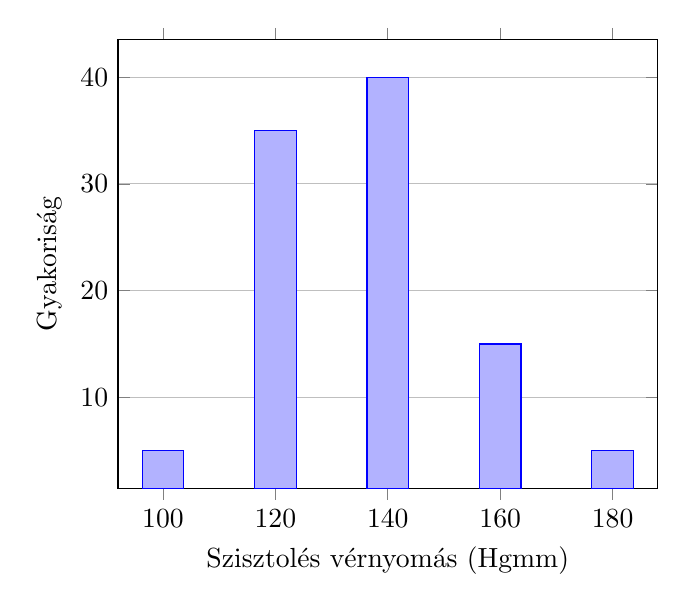
\begin{tikzpicture}
                \begin{axis}
                    [
                    ybar,
                    ylabel={Gyakoriság},
                    xlabel={Szisztolés vérnyomás (Hgmm)},
                    xtick={100,120,140,160,180},
                    ytick={0,10,20,30,40},
                    ymajorgrids=true,
                    bar width=15pt,
                    ]
                    \addplot coordinates {
                        (100,5) (120,35) (140,40) (160,15) (180,5)
                    };
                \end{axis}
            \end{tikzpicture}
        \end{center}

        Ez a hisztogram mutatja, hogy a legtöbb érték 120-140 Hgmm között van, és az eloszlás közel szimmetrikus.
    \end{description}

    \subsubsection{Magfüggvényes sűrűségbecslés}

    \begin{description}
        \item[Példa:] Ugyanazon vérnyomásadatok magfüggvényes sűrűségbecslése:

        \begin{center}
            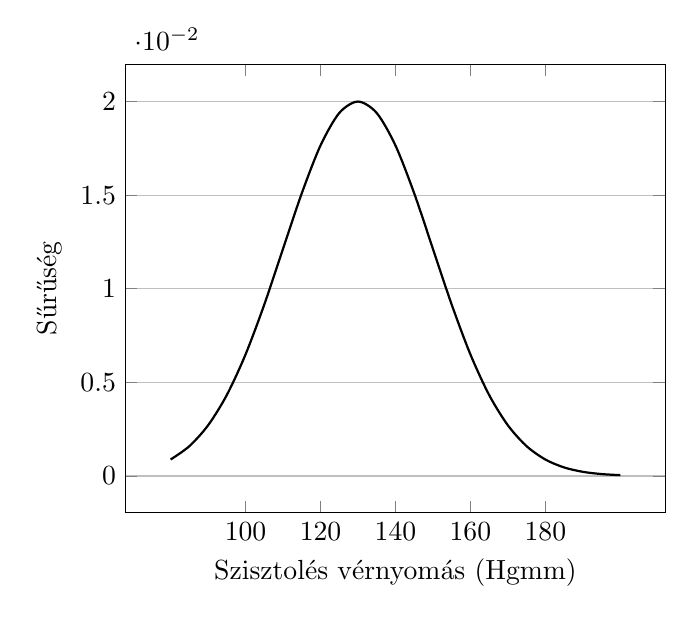
\begin{tikzpicture}
                \begin{axis}
                    [
                    ylabel={Sűrűség},
                    xlabel={Szisztolés vérnyomás (Hgmm)},
                    xtick={100,120,140,160,180},
                    ymajorgrids=true,
                    ]
                    \addplot[smooth, thick, domain=80:200] {0.02*exp(-0.5*((x-130)/20)^2)};
                \end{axis}
            \end{tikzpicture}
        \end{center}

        Ez a becslés simább képet ad az eloszlásról, mint a hisztogram, és jól mutatja az eloszlás csúcsát 130 Hgmm körül.
    \end{description}

    \subsubsection{Tukey-féle boxplot}

    A könyv a Low Infant Birth Weight (LOWBWT) adatbázis születési tömeg (bwt) változóját használja példaként a boxplot bemutatására.

    \begin{description}
        \item[Példa:] A LOWBWT adatbázis születési tömeg változójának boxplot ábrázolása:

        \begin{center}
            \begin{tikzpicture}
                \begin{axis}[
                    y=0.004cm,
                    boxplot/draw direction=y,
                    ylabel={Születési tömeg [g]},
                    ytick={1000,2000,3000,4000,5000},
                    height=8cm,
                    width=6cm
                ]
                    \addplot+[
                    boxplot prepared={
                        lower whisker=709,
                        lower quartile=2414,
                        median=2977,
                        upper quartile=3487,
                        upper whisker=4990
                    },
                    ] coordinates {};
                \end{axis}
            \end{tikzpicture}
        \end{center}

        A boxplot értelmezése:
        \begin{itemize}
            \item A doboz alja az első kvartilis (Q1 = 2414 g)
            \item A dobozban lévő vonal a medián (2977 g)
            \item A doboz teteje a harmadik kvartilis (Q3 = 3487 g)
            \item Az alsó "bajusz" vége a legkisebb nem kiugró érték (709 g)
            \item A felső "bajusz" vége a legnagyobb nem kiugró érték (4990 g)
        \end{itemize}

        Fontos megjegyzések:
        \begin{itemize}
            \item Az interkvartilis terjedelem (IQR) = Q3 - Q1 = 3487 - 2414 = 1073 g
            \item A boxplot nem mutat kiugró értékeket ebben a példában
            \item Az eloszlás enyhén jobbra ferde, mivel a medián közelebb van Q1-hez, mint Q3-hoz
        \end{itemize}
    \end{description}

    (Forrás: 32-33. oldal, 3.5. ábra)

    \subsection{Két folytonos változó együttes vizsgálata}

    Két folytonos változó kapcsolatának vizsgálatára több módszer is rendelkezésünkre áll. Ezek közül a legfontosabbak a kovariancia, a korreláció és a szóródási diagram.

    \subsubsection{Kovariancia}

    A kovariancia két változó együttes változékonyságát méri.

    \begin{equation}
        \text{cov}(x,y) = \frac{\sum_{i=1}^n (x_i - \bar{x})(y_i - \bar{y})}{n}
    \end{equation}

    \begin{description}
        \item[Értelmezés:]
        \begin{itemize}
            \item Pozitív kovariancia: a változók együtt mozognak
            \item Negatív kovariancia: a változók ellentétesen mozognak
            \item Nulla körüli kovariancia: nincs lineáris kapcsolat
        \end{itemize}
        \item[Hátrány:] Skálafüggő, nehezen összehasonlítható különböző változópárok között
    \end{description}

    (Forrás: 38-39. oldal)

    \subsubsection{Korreláció}

    A korreláció a kovariancia standardizált formája, amely -1 és +1 között mozog.

    \begin{equation}
        r = \frac{\text{cov}(x,y)}{s_x s_y}
    \end{equation}

    ahol $s_x$ és $s_y$ az $x$ és $y$ változók szórása.

    \begin{description}
        \item[Értelmezés:]
        \begin{itemize}
            \item $r = 1$: tökéletes pozitív lineáris kapcsolat
            \item $r = -1$: tökéletes negatív lineáris kapcsolat
            \item $r = 0$: nincs lineáris kapcsolat
        \end{itemize}
        \item[Előnyök:]
        \begin{itemize}
            \item Skálafüggetlen, összehasonlítható különböző változópárok között
            \item Könnyen értelmezhető
        \end{itemize}
        \item[Hátrányok:]
        \begin{itemize}
            \item Csak lineáris kapcsolatot mér
            \item Érzékeny a kiugró értékekre
        \end{itemize}
    \end{description}

    (Forrás: 39-40. oldal)

    \subsubsection{Szóródási diagram}

    A szóródási diagram két folytonos változó kapcsolatának grafikus ábrázolása.

    \begin{description}
        \item[Készítés:] Minden megfigyelési egységhez egy pontot rajzolunk egy derékszögű koordináta-rendszerben, ahol az x-koordináta az egyik, az y-koordináta a másik változó értéke.

        \item[Példa:] Tekintsük az anyai testtömeg (lwt) és az újszülött születési tömege (bwt) közötti kapcsolatot a LOWBWT adatbázisban:

        \begin{center}
            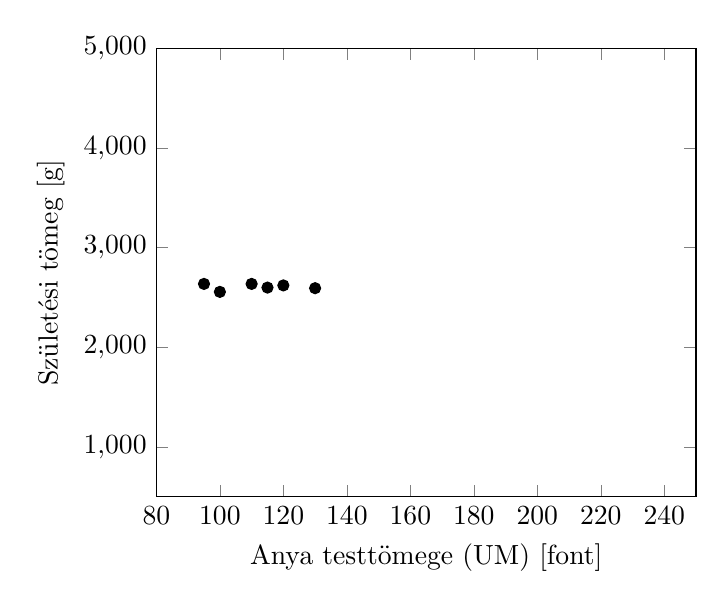
\begin{tikzpicture}
                \begin{axis}
                    [
                    xlabel={Anya testtömege (UM) [font]},
                    ylabel={Születési tömeg [g]},
                    xmin=80, xmax=250,
                    ymin=500, ymax=5000,
                    scatter/use mapped color={draw=black, fill=black},
                    ]
                    \addplot[only marks, scatter] table[x=lwt, y=bwt] {
                        lwt bwt
                        100 2557
                        130 2594
                        115 2600
                        120 2622
                        110 2637
                        95 2637
                    };
                \end{axis}
            \end{tikzpicture}
        \end{center}

        \item[Értelmezés:]
        \begin{itemize}
            \item A pontok elhelyezkedése mutatja a kapcsolat jellegét és erősségét
            \item Lineáris trend esetén a pontok egy egyenes mentén csoportosulnak
            \item A szórás mértéke az egyenes körül mutatja a kapcsolat erősségét
        \end{itemize}

        \item[Előnyök:]
        \begin{itemize}
            \item Vizuálisan jól értelmezhető
            \item Nemlineáris kapcsolatokat is kimutat
            \item Kiugró értékek könnyen azonosíthatók
        \end{itemize}
    \end{description}

    (Forrás: 40-41. oldal)

    \newpage


    \section{Következtető statisztitika alapjai}

    \paragraph{Tétel:} Minta és sokaság, a mintavételes helyzet fogalma. Véges és fiktív (végtelen) sokaságok.
    Mintavételi ingadozás és mintavételi hiba, szerepük az orvosi kutatásokban. A mintavételi hiba
    elleni védekezés alapgondolatai. Mintavételi és nem-mintavételi hiba.


    \section{Következtető statisztika alapjai}

    \subsection{Minta és sokaság, a mintavételes helyzet fogalma}

    \subsubsection{Sokaság (populáció)}

    A sokaság az a halmaz, amelyre a statisztikai eszközökkel megvizsgálandó kérdésünk vonatkozik.

    \begin{description}
        \item[Definíció:] A sokaság (vagy célpopuláció) az a halmaz, amelynek elemeiről információt szeretnénk nyerni.
        \item[Példa:] Ha azt kérdezzük, hogy "Mennyi egy adott kurzus hallgatóinak átlagos testtömege?", akkor a sokaság az adott kurzus hallgatóiból álló halmaz.
    \end{description}

    (Forrás: 7. oldal)

    \subsubsection{Minta}

    A minta a sokaság azon részhalmaza, amelyről ténylegesen információt gyűjtünk.

    \begin{description}
        \item[Definíció:] A minta a sokaság egy részhalmaza, amelyről adatokat gyűjtünk.
        \item[Példa:] Ha a kurzus 100 hallgatójából 30-at választunk ki véletlenszerűen és mérjük meg a testtömegüket, ez a 30 hallgató alkotja a mintát.
    \end{description}

    (Forrás: 7. oldal)

    \subsubsection{Mintavételes helyzet}

    Mintavételes helyzetről akkor beszélünk, amikor a sokaságnak csak egy részét tudjuk megfigyelni.

    \begin{description}
        \item[Okai:]
        \begin{itemize}
            \item Technikai okok: a teljes körű megfigyelés túl költséges, időigényes vagy bonyolult lehet.
            \item Fiktív sokaságok: sok kérdés nem egy kézzelfogható, véges nagyságú sokaságra vonatkozik.
        \end{itemize}
        \item[Jelentősége:] A biostatisztikában kiemelt fontosságú, mert gyakran dolgozunk fiktív sokaságokkal.
    \end{description}

    (Forrás: 7-8. oldal)

    \subsection{Véges és fiktív (végtelen) sokaságok}

    \subsubsection{Véges sokaságok}

    \begin{description}
        \item[Definíció:] Olyan sokaságok, amelyek elemei megszámlálhatók, véges számúak.
        \item[Példa:] Egy adott kurzus hallgatói, egy ország lakosai egy adott időpontban.
        \item[Jellemző:] Az elemek elvileg felsorolhatók, bár ez a gyakorlatban nem mindig kivitelezhető.
    \end{description}

    \subsubsection{Fiktív (végtelen) sokaságok}

    \begin{description}
        \item[Definíció:] Olyan sokaságok, amelyek elemei nem számlálhatók meg, vagy amelyek egy elméleti, végtelen populációt reprezentálnak.
        \item[Példa:] "Egy új vérnyomáscsökkentő gyógyszerjelölt valóban csökkenti-e a vérnyomást?" - itt a sokaság mindazok halmaza, akik potenciálisan használhatnák a gyógyszert.
        \item[Jellemző:] Nem lehet konkrétan felsorolni az elemeit, gyakran úgy tekintjük, mintha végtelen sok elem lenne benne.
    \end{description}(Forrás: 7-8. oldal)

    A fiktív sokaságok koncepciója különösen fontos a biostatisztikában, mert sok orvosi kutatás ilyen sokaságokra vonatkozik. Ezekben az esetekben bármilyen méretű minta is csak egy töredékét képviseli a teljes (elméleti) sokaságnak.

    \subsection{Mintavételi ingadozás és mintavételi hiba}

    \subsubsection{Mintavételi ingadozás}

    \begin{description}
        \item[Definíció:] A mintavételi ingadozás az a jelenség, amikor különböző minták különböző eredményeket adnak ugyanabból a sokaságból.

        \item[Magyarázat:] Bármilyen módszert is találunk ki arra, hogy a mintából hogyan következtessünk a sokaságra, annak a végeredménye mintáról-mintára változni fog, azaz függeni fog attól, hogy konkrétan hogyan vettünk mintát.

        \item[Példa:] Ha egy 1000 fős sokaságból veszünk egy 30 fős mintát a sokasági átlag becslésére, előfordulhat, hogy épp a 30 legkönnyebb embert választjuk ki, még tökéletesen véletlen mintavétel mellett is.
    \end{description}

    (Forrás: 46-47. oldal)

    Képzeljük el, hogy egy nagy zsák cukorkából csak néhányat veszünk ki, hogy megállapítsuk, milyen színűek a cukorkák a zsákban. Ha ezt többször megismételjük, valószínűleg minden alkalommal kicsit más eredményt kapunk. Ezt nevezzük mintavételi ingadozásnak.

    Ha egy 1000 fős városból megkérdezünk 30 embert a kedvenc színükről, majd ezt megismételjük egy másik 30 emberrel, valószínűleg kicsit eltérő eredményeket kapunk. Ez a mintavételi ingadozás.

    \subsubsection{Mintavételi hiba}

    \begin{description}
        \item[Definíció:] A mintavételi hiba az a hiba, amit a mintavételi ingadozás okoz a becslésünkben vagy következtetésünkben.

        \item[Jellemzők:]
        \begin{itemize}
            \item Elkerülhetetlen következménye a mintavételes helyzetnek.
            \item Statisztikai módszerekkel kezelhető és számszerűsíthető.
            \item Csökkenthető a mintaméret növelésével.
        \end{itemize}

        \item[Valószínűségi természet:] Bár nem tudjuk kizárni a nagy hibát, de meg tudjuk mondani, hogy ennek mennyi a valószínűsége.
    \end{description}
    (Forrás: 47. oldal)

    A mintavételi hiba az, amikor a kis mintánk alapján tévesen ítéljük meg az egész csoportot.

    Ha véletlenül csak olyan embereket kérdezünk meg a városban, akik mind kék ruhát viselnek, tévesen azt gondolhatnánk, hogy az egész városban mindenki szereti a kék színt. Ez lenne a mintavételi hiba.

    \subsubsection{Szerepük az orvosi kutatásokban}

    \begin{itemize}
        \item Az orvosi kutatásokban gyakran dolgozunk fiktív sokaságokkal, ahol a mintavételi ingadozás és hiba különösen fontos szerepet játszik.
        \item A kutatási eredmények értelmezésénél és általánosításánál figyelembe kell venni a mintavételi hiba lehetőségét.
        \item A statisztikai szignifikancia és a konfidencia intervallumok koncepciója a mintavételi hiba kezelésére szolgál.
    \end{itemize}

    Az orvosok gyakran nem tudják az összes létező beteget megvizsgálni, ezért kisebb csoportokon végeznek kutatásokat. A mintavételi ingadozás és hiba miatt fontos, hogy óvatosan vonjanak le következtetéseket.

    \subsection{A mintavételi hiba elleni védekezés alapgondolatai}

    \begin{enumerate}
        \item \textbf{Megfelelő mintavételi módszer:} Reprezentatív minta kiválasztása, amely jól tükrözi a sokaság tulajdonságait.

        \item \textbf{Mintaméret növelése:} Nagyobb minta általában csökkenti a mintavételi hibát.

        \item \textbf{Statisztikai módszerek alkalmazása:}
        \begin{itemize}
            \item Konfidencia intervallumok használata a becslés bizonytalanságának kifejezésére.
            \item Hipotézisvizsgálatok alkalmazása a véletlen ingadozások hatásának figyelembevételére.
        \end{itemize}

        \item \textbf{Ismételt vizsgálatok:} Ugyanazon kérdés vizsgálata többször, különböző mintákon.

        \item \textbf{Meta-analízis:} Több független kutatás eredményeinek összegzése a mintavételi hiba csökkentése érdekében.
    \end{enumerate}

    Fontos megérteni, hogy a mintavételi hiba teljesen nem küszöbölhető ki, de megfelelő módszerekkel és körültekintéssel jelentősen csökkenthető és kezelhető.

    (Forrás: 47-48. oldal)

    \textbf{Egyszerűsítve}:

    1. \textbf{Több embert vizsgálunk:} Minél többen vannak a mintában, annál pontosabb képet kapunk.

    2. \textbf{Véletlenszerűen választunk:} Így elkerülhetjük, hogy csak egy bizonyos típusú ember kerüljön a mintába.

    3. \textbf{Többször megismételjük a vizsgálatot:} Ha többször hasonló eredményt kapunk, biztosabbak lehetünk benne.

    4. \textbf{Statisztikai módszereket használunk:} Ezek segítenek megmondani, mennyire lehetünk biztosak az eredményeinkben.

    5. \textbf{Több kutatás eredményeit összehasonlítjuk:} Ha több különböző kutatás is hasonló eredményre jut, az megerősíti a következtetéseinket.

    Fontos tudni, hogy teljesen sosem tudjuk kiküszöbölni a mintavételi hibát, de ezekkel a módszerekkel jelentősen csökkenthetjük a hatását.

    \newpage


    \section{A következtető statisztika apparátusa: becsléselmélet}

    \paragraph{Tétel:} A becsléselmélet alapjai: becslőfüggvény, a becslőfüggvény mintavételi tulajdonságai
    (torzítatlanság, hatásosság, konzisztencia stb.). Pontbecslés és intervallumbecslés
    (konfidenciaintervallum). A mintanagyság szerepe és jelentősége, mintanagyság-tervezés.

    \subsection{A becsléselmélet alapjai}

    A becsléselmélet a következtető statisztika egyik fő ága, amelynek célja a sokaság jellemzőinek (paramétereinek) becslése a mintából nyert információk alapján.

    \paragraph{Magyarázat}
    Képzeljük el, hogy van egy hatalmas zsák cukorkánk, és szeretnénk tudni, átlagosan hány gramm egy cukorka ebben a zsákban. Nyilvánvalóan nem tudjuk az összes cukorkát megmérni, ezért csak néhányat veszünk ki és mérünk meg. Ez a folyamat a becslés lényege.

    \subsubsection{Becslőfüggvény}

    A becslőfüggvény olyan függvény, amelynek bemenetei a minta elemei, kimenete pedig a becsülni kívánt sokasági jellemző (paraméter) becslése.

    Formálisan: $\hat{\theta} = f(x_1, x_2, ..., x_n)$, ahol $\hat{\theta}$ a becsült érték, $\theta$ a becsülni kívánt paraméter, és $x_1, x_2, ..., x_n$ a mintaelemek.

    Ha a sokasági várható értéket ($\mu$) szeretnénk becsülni, egy lehetséges becslőfüggvény a mintaátlag:

    \[ \hat{\mu} = \bar{x} = \frac{1}{n}\sum_{i=1}^n x_i \]

    (Forrás: 47-48. oldal)

    \paragraph{Magyarázat}
    A becslőfüggvény olyan módszer, amivel a kis mintánkból (a kiválasztott cukorkákból) próbálunk következtetni az egész zsák tulajdonságaira.

    Ha azt szeretnénk megtudni, hogy átlagosan mennyi egy cukorka súlya, akkor megmérhetjük a kiválasztott cukorkákat, és kiszámolhatjuk ezek átlagát. Ez az átlagszámítás a becslőfüggvényünk.

    \subsubsection{A becslőfüggvény mintavételi tulajdonságai}

    \paragraph{Torzítatlanság}

    Egy becslőfüggvényt torzítatlannak nevezünk, ha a mintavételi eloszlásának várható értéke megegyezik a becsülni kívánt paraméter valódi értékével.

    Formálisan: $E(\hat{\theta}) = \theta$

    Ez azt jelenti, hogy a becslésünk "középértéke" hosszú távon megegyezik a valódi értékkel. Egyszerűbben: ha sokszor ismételnénk meg a becslést új mintákkal, az eredmények átlaga közel lenne a valódi értékhez.

    \paragraph{Hatásosság}

    Egy torzítatlan becslőfüggvényt hatásosnak nevezünk, ha a torzítatlan becslők körében minimális szórású.

    Egy hatásos becslés "közelebb" van a valódi értékhez, mint más becslések. Ha több módszerünk is van a becslésre, a hatásos az, amelyik általában a legpontosabb eredményt adja.

    \paragraph{Konzisztencia}
    Egy becslőfüggvény konzisztens, ha a mintaméret növekedésével a becslés egyre pontosabbá válik, azaz a becslés konvergál a valódi paraméterértékhez.

    Formálisan: $\lim_{n\to\infty} P\left(|\hat{\theta}_n - \theta| < \epsilon\right) = 1$ minden $\epsilon > 0$ esetén.

    Ahol:
    \begin{itemize}
        \item $\hat{\theta}_n$ a becslőfüggvény értéke $n$ mintaméret esetén
        \item $\theta$ a becsülni kívánt paraméter valódi értéke
        \item $\epsilon$ egy tetszőlegesen kicsi pozitív szám
        \item $P(\cdot)$ a valószínűséget jelöli
    \end{itemize}

    Ez a definíció azt jelenti, hogy ahogy a mintaméret tart a végtelenhez, annak a valószínűsége, hogy a becslés és a valódi érték közötti különbség abszolút értéke kisebb, mint bármely tetszőlegesen kicsi pozitív szám, 1-hez tart (azaz biztos eseménnyé válik).

    Ez azt jelenti, hogy minél több cukorkát veszünk ki a zsákból (azaz növeljük a mintaméretet), annál pontosabb lesz a becslésünk. Ha elég sok cukorkát mérnénk meg, szinte biztosan megkapnánk a helyes átlagsúlyt.

    \subsection{Pontbecslés és intervallumbecslés (konfidenciaintervallum)}

    \subsubsection{Pontbecslés}

    A pontbecslés egy statisztikai eljárás, amely során a minta adataiból egyetlen értéket számolunk ki a populáció ismeretlen paraméterének becslésére.

    \begin{itemize}
        \item A pontbecslés eredménye egy konkrét szám, amely a becsülni kívánt paraméter "legjobb becslése".
        \item Általában valamilyen mintastatisztikát használunk pontbecslésként, például a mintaátlagot vagy a mintaarányt.
    \end{itemize}

    \paragraph{Példa:} Ha a populáció átlagéletkorát szeretnénk becsülni, és egy 100 fős mintában az átlagéletkor 45 év, akkor a populáció átlagéletkorának pontbecslése 45 év.

    \paragraph{A pontbecslés korlátai:}
    \begin{itemize}
        \item Nem ad információt a becslés pontosságáról vagy megbízhatóságáról.
        \item Nem veszi figyelembe a mintavételi ingadozást.
    \end{itemize}

    \subsubsection{Intervallumbecslés (konfidenciaintervallum)}

    \paragraph{Definíció}
    Az intervallumbecslés során egy intervallumot határozunk meg, amely adott valószínűséggel (konfidenciaszint) tartalmazza a becsülni kívánt paramétert.

    \paragraph{A konfidenciaintervallum fő jellemzői:}
    \begin{itemize}
        \item Két értéket ad meg: egy alsó és egy felső határt.
        \item Tartalmaz egy valószínűségi állítást (konfidenciaszint), általában 95\% vagy 99\%.
        \item Figyelembe veszi a mintavételi ingadozást és a becslés bizonytalanságát.
    \end{itemize}

    \paragraph{Példa}
    Ha a fenti példában a 45 éves átlagéletkor 95\%-os konfidenciaintervalluma (42 év, 48 év), akkor ezt így értelmezzük: ha sokszor megismételnénk a mintavételt és minden alkalommal kiszámolnánk ezt az intervallumot, az esetek 95\%-ában tartalmazná a valódi populációs átlagot.

    \paragraph{A konfidenciaintervallum általános formája:}
    \[ \text{Pontbecslés} \pm (\text{Kritikus érték}) \cdot (\text{A becslés standard hibája}) \]

    \paragraph{A konfidenciaintervallum értelmezése:}
    \begin{itemize}
        \item Nem azt jelenti, hogy a paraméter 95\% valószínűséggel esik az intervallumba.
        \item Azt fejezi ki, hogy ha sokszor megismételnénk a mintavételt, az intervallumok 95\%-a tartalmazná a valódi paramétert.
    \end{itemize}

    \subsubsection{Összehasonlítás}

    \begin{tabular}{|l|l|l|}
        \hline
        Jellemző                                 & Pontbecslés      & Intervallumbecslés \\
        \hline
        Eredmény formája                         & Egyetlen szám    & Intervallum        \\
        Bizonytalanság kifejezése                & Nem              & Igen               \\
        Mintavételi ingadozás kezelése           & Nem              & Igen               \\
        Értelmezés egyszerűsége                  & Egyszerűbb       & Összetettebb       \\
        Statisztikai következtetésre alkalmasság & Kevésbé alkalmas & Alkalmasabb        \\
        \hline
    \end{tabular}

    \paragraph{Megjegyzés}
    Bár a pontbecslés egyszerűbb és közvetlenebb, az intervallumbecslés általában informatívabb és jobban tükrözi a statisztikai következtetés bizonytalanságát. A gyakorlatban gyakran mindkettőt megadják: a pontbecslést mint a "legjobb becslést", és a konfidenciaintervallumot mint a becslés megbízhatóságának mértékét.

    \subsection{Pontbecslés és intervallumbecslés (konfidenciaintervallum)}

    Képzeljük el, hogy egy nagy tó halainak átlagos súlyát szeretnénk megbecsülni, de nem tudjuk az összes halat megmérni.

    \subsubsection{Pontbecslés}

    A pontbecslés olyan, mintha kifogtunk volna néhány halat, megmértük volna őket, és az átlagukat használnánk a tó összes halának átlagos súlyaként. Tegyük fel, hogy kifogtunk 50 halat, és ezek átlagos súlya 300 gramm. Ekkor azt mondanánk, hogy becslésünk szerint a tó halainak átlagos súlya 300 gramm.


    A pontbecslés egy statisztikai eljárás, amely során a minta adataiból egyetlen értéket számolunk ki a populáció ismeretlen paraméterének becslésére.

    \begin{itemize}
        \item A pontbecslés eredménye egy konkrét szám, amely a becsülni kívánt paraméter "legjobb becslése".
        \item Általában valamilyen mintastatisztikát használunk pontbecslésként, például a mintaátlagot vagy a mintaarányt.
    \end{itemize}

    \paragraph{Példa:}
    Ha a populáció átlagéletkorát szeretnénk becsülni, és egy 100 fős mintában az átlagéletkor 45 év, akkor a populáció átlagéletkorának pontbecslése 45 év.

    \paragraph{A pontbecslés korlátai:}
    \begin{itemize}
        \item Nem ad információt a becslés pontosságáról vagy megbízhatóságáról.
        \item Nem veszi figyelembe a mintavételi ingadozást.
    \end{itemize}

    \paragraph{A pontbecslés előnyei és hátrányai:}
    \begin{itemize}
        \item Előny: Egyszerű, könnyen érthető.
        \item Hátrány: Nem mutatja, mennyire lehetünk biztosak ebben a becslésben.
    \end{itemize}

    \subsubsection{Intervallumbecslés (konfidenciaintervallum)}

    Az intervallumbecslés során egy intervallumot határozunk meg, amely adott valószínűséggel (konfidenciaszint) tartalmazza a becsülni kívánt paramétert.

    Az intervallumbecslés olyan, mintha azt mondanánk: "Nem vagyunk biztosak a pontos átlagban, de nagy valószínűséggel ebben a tartományban van." Ahelyett, hogy csak annyit mondanánk, hogy az átlagos súly 300 gramm, azt mondhatnánk: "95\% biztos vagyok benne, hogy a tó halainak átlagos súlya 280 és 320 gramm között van."

    \paragraph{A konfidenciaintervallum fő jellemzői:}
    \begin{itemize}
        \item Két értéket ad meg: egy alsó és egy felső határt.
        \item Tartalmaz egy valószínűségi állítást (konfidenciaszint), általában 95\% vagy 99\%. egmondja, mennyire lehetünk biztosak ebben a tartományban (pl. 95\% biztos).
        \item Figyelembe veszi a mintavételi ingadozást és a becslés bizonytalanságát. Figyelembe veszi, hogy a becslésünk nem tökéletes.
    \end{itemize}

    \paragraph{Példa}
    Ha a fenti példában a 45 éves átlagéletkor 95\%-os konfidenciaintervalluma (42 év, 48 év), akkor ezt így értelmezzük: ha sokszor megismételnénk a mintavételt és minden alkalommal kiszámolnánk ezt az intervallumot, az esetek 95\%-ában tartalmazná a valódi populációs átlagot.

    \paragraph{A konfidenciaintervallum általános formája:}
    \[ \text{Pontbecslés} \pm (\text{Kritikus érték}) \cdot (\text{A becslés standard hibája}) \]

    \paragraph{A konfidenciaintervallum értelmezése:}
    \begin{itemize}
        \item Nem azt jelenti, hogy a paraméter 95\% valószínűséggel esik az intervallumba.
        \item Azt fejezi ki, hogy ha sokszor megismételnénk a mintavételt, az intervallumok 95\%-a tartalmazná a valódi paramétert.
    \end{itemize}

    \subsubsection{Összehasonlítás}

    \begin{tabular}{|l|l|l|}
        \hline
        Jellemző                                 & Pontbecslés      & Intervallumbecslés \\
        \hline
        Eredmény formája                         & Egyetlen szám    & Intervallum        \\
        Bizonytalanság kifejezése                & Nem              & Igen               \\
        Mintavételi ingadozás kezelése           & Nem              & Igen               \\
        Értelmezés egyszerűsége                  & Egyszerűbb       & Összetettebb       \\
        Statisztikai következtetésre alkalmasság & Kevésbé alkalmas & Alkalmasabb        \\
        \hline
    \end{tabular}

    Miért jobb az intervallumbecslés?
    \textbf{Őszintébb:} Elismeri, hogy nem lehetünk teljesen biztosak a becslésünkben.

    \textbf{Informatívabb:} Megmutatja, mennyire pontos vagy pontatlan a becslésünk.

    \textbf{Biztonságosabb döntésekhez vezet:} Ha tudjuk a lehetséges tartományt, óvatosabban tervezhetünk.


    Bár a pontbecslés egyszerűbb és közvetlenebb, az intervallumbecslés általában informatívabb és jobban tükrözi a statisztikai következtetés bizonytalanságát. A gyakorlatban gyakran mindkettőt megadják: a pontbecslést mint a "legjobb becslést", és a konfidenciaintervallumot mint a becslés megbízhatóságának mértékét.

    Összehasonlítás egyszerű példával
    Képzeljük el, hogy meg akarjuk becsülni egy barátunk életkorát:
    \begin{itemize}
        \item Pontbecslés: "Szerintem 35 éves."
        \item Intervallumbecslés: "Elég biztos vagyok benne, hogy 32 és 38 év között van."
    \end{itemize}
    Az intervallumbecslés több információt ad, és jobban kifejezi a bizonytalanságunkat.

    A statisztikusok gyakran mindkettőt használják: a pontbecslést mint legjobb tippet, és az intervallumbecslést, hogy megmutassák, mennyire biztosak ebben a tippben.

    \subsection{A mintanagyság szerepe és jelentősége, mintanagyság-tervezés}

    \subsubsection{A mintanagyság szerepe}

    A mintanagyság kritikus tényező a statisztikai következtetések megbízhatóságában és pontosságában. Hatása több aspektusban is megmutatkozik:

    \paragraph{Becslések pontossága}
    A mintanagyság növelésével általában javul a becslések pontossága. Ezt matematikailag a standard hiba fogalmával ragadhatjuk meg:

    \[ SE = \frac{\sigma}{\sqrt{n}} \]

    ahol $SE$ a standard hiba, $\sigma$ a populáció szórása, és $n$ a mintanagyság.

    \textbf{Szemléletes magyarázat:} Gondoljunk úgy a kutatásra, mint amikor levest kóstolunk. Ha csak egy kanállal kóstolunk, lehet, hogy épp egy olyan részt fogtunk ki, ami nem jellemző az egész fazékra. Minél több kanállal kóstolunk (azaz minél nagyobb a mintánk), annál biztosabbak lehetünk abban, hogy tudjuk, milyen az egész fazék leves (azaz a teljes populáció).

    \paragraph{Konfidenciaintervallumok szélessége}
    A mintanagyság közvetlenül befolyásolja a konfidenciaintervallumok szélességét. Nagyobb minta általában szűkebb konfidenciaintervallumot eredményez, ami precízebb becslést jelent.

    \textbf{Szemléletes magyarázat:} Ha azt mondjuk, "a leves valahol 70 és 80 fok között van", az jobb, mint csak tippelni. Több ember bevonásával (nagyobb mintával) szűkíthetjük ezt a tartományt, például "73 és 77 fok között".

    \paragraph{Statisztikai próbák ereje}
    A mintanagyság növelésével nő a statisztikai próbák ereje, azaz a valódi különbségek detektálásának képessége.

    \textbf{Szemléletes magyarázat:} Ha csak pár embert vizsgálunk, csak a nagy különbségeket vesszük észre. Több emberrel a kisebb, finomabb különbségeket is észlelhetjük. Ez olyan, mintha egy homályos fényképet néznénk - több adat (nagyobb minta) esetén élesebb lesz a kép.

    \subsubsection{Mintanagyság-tervezés}

    A mintanagyság-tervezés a kutatás tervezési fázisának kulcsfontosságú eleme. Célja annak meghatározása, mekkora mintára van szükség egy adott kutatási kérdés megválaszolásához.

    \textbf{Szemléletes magyarázat:} Ez olyan, mint amikor pizzát rendelünk egy bulira. Túl kevés pizza = éhes vendégek (nem megbízható eredmények). Túl sok pizza = pazarlás (felesleges erőforrás-felhasználás). Meg kell találnunk az arany középutat.

    \paragraph{Főbb szempontok a mintanagyság meghatározásában}

    \begin{enumerate}
        \item \textbf{Kívánt pontosság:} Milyen mértékű pontosságot szeretnénk elérni a becsléseinkben?
        \item \textbf{Várható hatásnagyság:} Mekkora különbséget vagy összefüggést várunk?
        \textbf{Szemléletes magyarázat:} Ha azt akarjuk tudni, van-e különbség a 10 és 100 kilós emberek között, kevesebb ember elég. Ha a 70 és 75 kilósokat hasonlítjuk, több kell.
        \item \textbf{Statisztikai erő:} Általában 80\% vagy 90\% erőt céloznak meg a kutatások.
        \item \textbf{Szignifikanciaszint:} Tipikusan 5\% ($\alpha = 0.05$).
        \item \textbf{Variabilitás:} A vizsgált változó(k) várható szórása.
        \textbf{Szemléletes magyarázat:} Ha mindenki nagyon hasonló, kevesebb ember elég. Ha nagy a változatosság, több kell.
        \item \textbf{Elemzési módszer:} Különböző statisztikai módszerek eltérő mintanagyságot igényelhetnek.
    \end{enumerate}

    \paragraph{Mintanagyság-számítás}
    A mintanagyság-számítás általános formulája:

    \[ n = f(\alpha, \beta, \delta, \sigma) \]

    ahol $\alpha$ a szignifikanciaszint, $\beta$ a II. típusú hiba valószínűsége (1 - statisztikai erő), $\delta$ a detektálni kívánt hatás nagysága, és $\sigma$ a populáció szórása.

    \paragraph{Gyakorlati megfontolások}

    \begin{itemize}
        \item \textbf{Erőforrás-korlátok:} Idő, költség, személyzet rendelkezésre állása.
        \item \textbf{Etikai szempontok:} Minimálisan szükséges résztvevők száma.
        \item \textbf{Lemorzsolódás:} Figyelembe kell venni a várható lemorzsolódási arányt.
        \item \textbf{Alcsoportelemzések:} Ha tervezünk alcsoportelemzéseket, az növelheti a szükséges mintanagyságot.
    \end{itemize}

    \subsubsection{Mintanagyság és a statisztikai következtetések megbízhatósága}

    A megfelelő mintanagyság kiválasztása kritikus a statisztikai következtetések megbízhatósága szempontjából:

    \begin{itemize}
        \item \textbf{Túl kis minta:} Alacsony statisztikai erő, nagy konfidenciaintervallumok, megbízhatatlan becslések.
        \textbf{Szemléletes magyarázat:} Olyan, mintha rossz szemüveggel próbálnánk olvasni. Nem látjuk tisztán a képet, és lehet, hogy fontos dolgokat nem veszünk észre.
        \item \textbf{Túl nagy minta:} Felesleges erőforrás-pazarlás, etikai kérdések.
        \textbf{Szemléletes magyarázat:} Mintha kalapáccsal próbálnánk szöget beverni egy képbe. Túlzás, pazarlás, és esetleg több embert teszünk ki felesleges kockázatnak.
        \item \textbf{Optimális mintanagyság:} Egyensúly a statisztikai megbízhatóság és a gyakorlati megvalósíthatóság között.
    \end{itemize}

    \subsubsection{Konklúzió}

    A mintanagyság-tervezés alapvető fontosságú a kutatás megbízhatósága és érvényessége szempontjából. A megfelelően megválasztott mintanagyság biztosítja, hogy a kutatás elegendő statisztikai erővel rendelkezzen a valós hatások detektálásához, miközben elkerüli a felesleges erőforrás-pazarlást.

    \textbf{Szemléletes összefoglalás:} A megfelelő számú ember kiválasztása olyan, mint a jó szakács munkája: elég hozzávalót használ, hogy finom legyen az étel, de nem pazarol. Jó kutatáshoz meg kell találnunk az egyensúlyt a megbízhatóság és a gyakorlati megvalósíthatóság között.

    \newpage


    \section{A következtető statisztika apparátusa: hipotézisvizsgálat}

    \paragraph{Tétel:}A hipotézisvizsgálat alapfogalmai, null- és ellenhipotézis, tesztstatisztika. A hipotézisvizsgálat
    logikája. Első- és másodfajú hiba. Döntés hipotézisvizsgálatban: szignifikanciaszint, kritikus
    érték, p-érték. Egy- és kétoldalú próbák. Próba választása adott kérdés vizsgálatára.

    \subsection{A hipotézisvizsgálat alapfogalmai}

    A hipotézisvizsgálat a következtető statisztika egyik fő ága, amely lehetővé teszi, hogy mintából származó adatok alapján következtetéseket vonjunk le a populációra vonatkozóan.

    \subsubsection{Null- és ellenhipotézis}

    \paragraph{Definíció:}
    \begin{itemize}
        \item \textbf{Nullhipotézis ($H_0$):} Az a feltételezés, amelyet vizsgálni szeretnénk, általában egy "nincs különbség" vagy "nincs hatás" típusú állítás.
        \item \textbf{Ellenhipotézis ($H_1$):} A nullhipotézis tagadása, általában az az állítás, amit bizonyítani szeretnénk.
    \end{itemize}

    \textbf{Laikus magyarázat:}
    Képzeljük el, hogy egy új gyógyszert tesztelünk. A nullhipotézis olyan, mintha azt mondanánk: "Ez a gyógyszer nem jobb, mint a placebo". Az ellenhipotézis pedig: "Ez a gyógyszer hatásosabb, mint a placebo". A hipotézisvizsgálat során megpróbáljuk eldönteni, melyik állítás valószínűbb az adataink alapján.

    \paragraph{Példa:}
    $H_0: \mu = \mu_0$ (a populáció átlaga egyenlő egy adott értékkel)
    $H_1: \mu \neq \mu_0$ (a populáció átlaga nem egyenlő ezzel az értékkel)

    (Forrás: 55-56. oldal)

    \subsubsection{Tesztstatisztika}

    \paragraph{Definíció:}
    A tesztstatisztika egy olyan függvény, amely a minta adataiból számolható, és amelynek eloszlása ismert a nullhipotézis fennállása esetén.

    \textbf{Laikus magyarázat:}
    A tesztstatisztika olyan, mint egy mérőszám, amit az adatainkból számolunk ki. Ez a szám segít eldönteni, hogy mennyire valószínű, hogy a nullhipotézis igaz. Minél szélsőségesebb (nagyobb vagy kisebb) ez a szám, annál valószínűbb, hogy a nullhipotézis nem igaz.

    \paragraph{Példa:}
    Egy gyakran használt tesztstatisztika a t-statisztika:

    \[ t = \frac{\bar{x} - \mu_0}{s / \sqrt{n}} \]

    ahol $\bar{x}$ a mintaátlag, $\mu_0$ a nullhipotézisben szereplő érték, $s$ a minta szórása, és $n$ a mintaméret.

    \textbf{Laikus magyarázat:}
    Gondoljunk erre úgy, mint egy "különbségmérő"-re. Azt mutatja meg, hogy a mintánk átlaga mennyire tér el attól, amit a nullhipotézis állít, figyelembe véve, hogy mennyire változékonyak az adataink és hány adatpontunk van.

    (Forrás: 57-58. oldal)

    \subsubsection{A tesztstatisztika eloszlása}

    A nullhipotézis fennállása esetén a tesztstatisztika eloszlása ismert. Ez teszi lehetővé, hogy meghatározzuk, mennyire valószínű vagy valószínűtlen a kapott eredmény, ha a nullhipotézis igaz.

    \textbf{Laikus magyarázat:}
    Ez olyan, mintha tudnánk, hogy normál körülmények között (amikor a nullhipotézis igaz) milyen értékeket szokott felvenni a "különbségmérőnk". Ha olyan értéket kapunk, ami nagyon ritka normál körülmények között, az arra utal, hogy talán mégsem a nullhipotézis az igaz.

    A hipotézisvizsgálat alapfogalmainak megértése kulcsfontosságú a statisztikai következtetések helyes értelmezéséhez. Ezek az eszközök lehetővé teszik, hogy objektív módon értékeljük az adatainkat és döntéseket hozzunk tudományos kérdésekben.

    \subsection{A hipotézisvizsgálat logikája}

    A hipotézisvizsgálat egy indirekt bizonyítási módszer, amely a nullhipotézis cáfolatára törekszik.

    \subsubsection{A hipotézisvizsgálat lépései}

    \begin{enumerate}
        \item Nullhipotézis ($H_0$) és ellenhipotézis ($H_1$) megfogalmazása
        \item Szignifikanciaszint ($\alpha$) megválasztása
        \item Megfelelő tesztstatisztika kiválasztása
        \item Tesztstatisztika kiszámítása a mintából
        \item Döntés a nullhipotézis elutasításáról vagy el nem utasításáról
    \end{enumerate}

    (Forrás: 59-60. oldal)

    \subsubsection{A hipotézisvizsgálat logikájának részletes magyarázata}

    \paragraph{1. Feltételezés:}
    Kiindulásként feltételezzük, hogy a nullhipotézis igaz.

    \paragraph{2. Valószínűség-számítás:}
    Kiszámítjuk, hogy ha a nullhipotézis igaz lenne, milyen valószínűséggel kapnánk a megfigyelthez hasonló vagy még szélsőségesebb eredményt.

    \paragraph{3. Következtetés:}
    Ha ez a valószínűség nagyon kicsi (általában kisebb, mint az előre meghatározott szignifikanciaszint), akkor elutasítjuk a nullhipotézist, és az ellenhipotézist fogadjuk el.

    \textbf{Laikus magyarázat:}
    Képzeljük el, hogy egy érmével dobálunk, és azt állítjuk, hogy az érme szabályos (ez a nullhipotézis). Ha 100 dobásból 90-szer fejet kapunk, ez annyira valószínűtlen egy szabályos érme esetén, hogy inkább arra következtetünk, hogy az érme nem szabályos (elutasítjuk a nullhipotézist).

    \subsubsection{A hipotézisvizsgálat paradoxona}

    A hipotézisvizsgálat nem bizonyítja be az ellenhipotézis igazságát, csak a nullhipotézis valószínűtlenségét mutatja meg.

    \textbf{Laikus magyarázat:}
    Ez olyan, mintha egy bírósági tárgyaláson nem azt próbálnánk bizonyítani, hogy a vádlott bűnös, hanem azt, hogy nagyon valószínűtlen, hogy ártatlan. Ha sikerül megmutatni, hogy az ártatlanság nagyon valószínűtlen, akkor a bíróság bűnösnek nyilvánítja a vádlottat.

    \subsubsection{A hipotézisvizsgálat erőssége és gyengesége}

    \paragraph{Erősség:}
    Objektív módszert biztosít a tudományos állítások értékelésére.

    \paragraph{Gyengeség:}
    Nem ad információt a hatás nagyságáról, csak annak statisztikai szignifikanciájáról.

    \textbf{Laikus magyarázat:}
    Ez olyan, mintha azt tudnánk megmondani, hogy egy különbség "valódi" vagy sem, de azt nem, hogy ez a különbség mennyire fontos vagy jelentős a gyakorlatban.

    A hipotézisvizsgálat logikájának megértése kulcsfontosságú a statisztikai eredmények helyes értelmezéséhez. Fontos tudni, hogy a statisztikai szignifikancia nem feltétlenül jelent gyakorlati jelentőséget, és a nullhipotézis el nem utasítása nem jelenti annak bizonyítását.

    (Forrás: 60-62. oldal)

    \subsection{Hibák a hipotézisvizsgálatban}

    A hipotézisvizsgálat során kétféle hibát követhetünk el: elsőfajú és másodfajú hibát.

    \subsubsection{Elsőfajú hiba}

    \paragraph{Definíció:}
    Elsőfajú hibát akkor követünk el, ha elutasítjuk a nullhipotézist, amikor az valójában igaz.

    \paragraph{Jelölés:} $\alpha$ (alfa)

    \paragraph{Értelmezés:}
    Az elsőfajú hiba valószínűsége megegyezik a választott szignifikanciaszinttel.

    \textbf{Laikus magyarázat:}
    Ez olyan, mintha tévesen bűnösnek nyilvánítanánk egy ártatlan embert. Például, ha azt állítjuk, hogy egy új gyógyszer hatásos, amikor valójában nem az.

    (Forrás: 63-64. oldal)

    \subsubsection{Másodfajú hiba}

    \paragraph{Definíció:}
    Másodfajú hibát akkor követünk el, ha nem utasítjuk el a nullhipotézist, amikor az valójában hamis.

    \paragraph{Jelölés:} $\beta$ (béta)

    \paragraph{Értelmezés:}
    A másodfajú hiba valószínűsége függ a valódi hatás nagyságától és a mintamérettől.

    \textbf{Laikus magyarázat:}
    Ez olyan, mintha felmentenénk egy bűnös embert. Például, ha azt állítjuk, hogy egy új gyógyszer nem hatásos, amikor valójában az.

    (Forrás: 64-65. oldal)

    \subsubsection{A próba ereje}

    \paragraph{Definíció:}
    A próba ereje annak a valószínűsége, hogy elutasítjuk a nullhipotézist, amikor az valóban hamis.

    \paragraph{Jelölés:} $1 - \beta$

    \paragraph{Értelmezés:}
    A próba ereje azt mutatja meg, milyen valószínűséggel tudjuk detektálni a valódi hatást.

    \textbf{Laikus magyarázat:}
    Ez olyan, mint egy detektor érzékenysége. Minél nagyobb az erő, annál valószínűbb, hogy észrevesszük a valódi különbséget vagy hatást, ha az tényleg létezik.

    (Forrás: 65-66. oldal)

    \subsubsection{Az elsőfajú és másodfajú hiba összefüggése}

    \begin{itemize}
        \item Az elsőfajú hiba csökkentése általában növeli a másodfajú hiba valószínűségét és fordítva.
        \item A mintaméret növelése mind az elsőfajú, mind a másodfajú hiba valószínűségét csökkenti.
    \end{itemize}

    \textbf{Laikus magyarázat:}
    Ez olyan, mint amikor egy biztonsági rendszert állítunk be. Ha túl érzékenyre állítjuk, sok hamis riasztást kapunk (elsőfajú hiba), ha túl kevéssé érzékenyre, akkor viszont igazi betöréseket nem észlelünk (másodfajú hiba). A jó egyensúly megtalálása a cél.

    \begin{table}
        \centering
        \begin{tabular}{|c|c|c|}
            \hline
            & $H_0$ igaz                   & $H_0$ hamis                 \\
            \hline
            $H_0$ elutasítása & Elsőfajú hiba ($\alpha$)     & Helyes döntés (1 - $\beta$) \\
            \hline
            $H_0$ elfogadása  & Helyes döntés (1 - $\alpha$) & Másodfajú hiba ($\beta$)    \\
            \hline
        \end{tabular}
        \caption{A hipotézisvizsgálat lehetséges kimenetelei}
    \end{table}

    A hipotézisvizsgálat során mindig fennáll a hibázás lehetősége. A cél az, hogy mindkét típusú hiba valószínűségét elfogadhatóan alacsony szinten tartsuk. Ez általában kompromisszumot igényel a két hibatípus között, figyelembe véve a kutatás céljait és a lehetséges következményeket.

    (Forrás: 66-67. oldal)

    \subsection{Döntés hipotézisvizsgálatban: szignifikanciaszint, kritikus érték, p-érték}

    A hipotézisvizsgálat során a döntéshozatal három kulcsfogalom köré épül: szignifikanciaszint, kritikus érték és p-érték. Ezek segítségével tudjuk eldönteni, hogy elutasítjuk-e a nullhipotézist vagy sem.

    \subsubsection{Szignifikanciaszint ($\alpha$)}

    A szignifikanciaszint az a küszöbérték, amelynél kisebb p-érték esetén elutasítjuk a nullhipotézist.

    \begin{itemize}
        \item Általában használt értékek: 0,05 (5\%) vagy 0,01 (1\%)
        \item Jelölése: $\alpha$ (alfa)
    \end{itemize}

    \paragraph{Szakmai magyarázat:} A szignifikanciaszint az elsőfajú hiba elkövetésének maximális valószínűsége, amit még elfogadhatónak tartunk. Az elsőfajú hiba az, amikor elutasítjuk a nullhipotézist, pedig az valójában igaz.

    \paragraph{Laikus magyarázat:} Képzeljük el, hogy egy bíróságon vagyunk. A szignifikanciaszint olyan, mint amikor előre megmondjuk, hogy maximum hány százalékban vagyunk hajlandóak tévedni, amikor valakit bűnösnek nyilvánítunk. Ha 5\%-os szignifikanciaszintet választunk, az azt jelenti, hogy 100 esetből maximum 5-ször vagyunk hajlandóak tévedni.

    \subsubsection{Kritikus érték}

    A kritikus érték az a határérték, amelynél szélsőségesebb tesztstatisztika érték esetén elutasítjuk a nullhipotézist.

    \paragraph{Szakmai magyarázat:} A kritikus értéket a választott szignifikanciaszint és a tesztstatisztika nullhipotézis szerinti eloszlása alapján határozzuk meg. Ha a tesztstatisztika abszolút értéke nagyobb, mint a kritikus érték, elutasítjuk a nullhipotézist.

    \paragraph{Laikus magyarázat:} Gondoljunk a kritikus értékre úgy, mint egy sebességkorlátra. Ha valaki gyorsabban hajt ennél, akkor ``elutasítjuk'' azt az állítást, hogy betartja a sebességhatárt. A kritikus érték az a pont, ahol meghúzzuk a határt a ``még elfogadható'' és a ``már túl szélsőséges'' eredmények között.

    \subsubsection{p-érték}

    A p-érték annak a valószínűsége, hogy a nullhipotézis fennállása esetén a megfigyelthez hasonló vagy annál szélsőségesebb eredményt kapunk.

    \paragraph{Szakmai magyarázat:} Ha a p-érték kisebb, mint a választott szignifikanciaszint, akkor elutasítjuk a nullhipotézist. A p-érték nem a nullhipotézis igazságának valószínűségét adja meg, hanem azt mutatja, mennyire összeegyeztethető a megfigyelt adat a nullhipotézissel.

    \paragraph{Laikus magyarázat:} A p-érték olyan, mint egy ``meglepetésmérő''. Ha nagyon kicsi a p-érték, az azt jelenti, hogy az eredményünk nagyon meglepő lenne, ha a nullhipotézis igaz lenne. Például, ha egy érme dobálásakor 100-ból 99-szer fejet kapunk, a p-érték nagyon kicsi lenne, mert ez rendkívül meglepő eredmény lenne egy szabályos érme esetén.

    \subsubsection{Összehasonlítás és döntési folyamat}

    A hipotézisvizsgálat során általában két módszert használhatunk a döntéshozatalra:

    \begin{enumerate}
        \item \textbf{Kritikus érték módszer:} Összehasonlítjuk a tesztstatisztika értékét a kritikus értékkel. Ha a tesztstatisztika abszolút értéke nagyobb, mint a kritikus érték, elutasítjuk a nullhipotézist.

        \item \textbf{p-érték módszer:} Összehasonlítjuk a p-értéket a szignifikanciaszinttel. Ha a p-érték kisebb, mint a szignifikanciaszint, elutasítjuk a nullhipotézist.
    \end{enumerate}

    \paragraph{Laikus magyarázat:} Képzeljük el, hogy egy nyomozást folytatunk. A kritikus érték módszer olyan, mintha előre meghatároznánk, hogy milyen erős bizonyíték kell a gyanúsított letartóztatásához. A p-érték módszer pedig olyan, mintha minden esetben megvizsgálnánk, mennyire gyanús a bizonyíték, és összehasonlítanánk egy előre meghatározott ``gyanússági küszöbbel''.

    Fontos megjegyezni, hogy bár ezek a módszerek segítenek a döntéshozatalban, önmagukban nem elegendőek a tudományos következtetések levonásához. Mindig figyelembe kell venni a hatás nagyságát, a gyakorlati jelentőséget és az eredmények reprodukálhatóságát is.

    \subsection{Egy- és kétoldalú próbák}

    \subsubsection{Definíciók és jellemzők}

    \paragraph{Egyoldalú próba:}
    \begin{itemize}
        \item Az ellenhipotézis csak egyik irányú eltérést fogalmaz meg (nagyobb vagy kisebb).
        \item Példa nullhipotézis: $H_0: \mu \leq \mu_0$
        \item Példa ellenhipotézis: $H_1: \mu > \mu_0$
        \item Az elutasítási tartomány csak az eloszlás egyik szélén található.
    \end{itemize}

    \paragraph{Kétoldalú próba:}
    \begin{itemize}
        \item Az ellenhipotézis mindkét irányú eltérést megengedi.
        \item Példa nullhipotézis: $H_0: \mu = \mu_0$
        \item Példa ellenhipotézis: $H_1: \mu \neq \mu_0$
        \item Az elutasítási tartomány az eloszlás mindkét szélén megtalálható.
    \end{itemize}

    \subsubsection{Különbségek}
    \begin{itemize}
        \item Az egyoldalú próba esetén a kritikus érték kevésbé szélsőséges, mint a kétoldalú próbánál azonos szignifikanciaszint mellett.
        \item Az egyoldalú próba nagyobb statisztikai erővel rendelkezik, ha a feltételezés helyes az eltérés irányáról.
        \item A kétoldalú próba általánosabb és biztonságosabb, ha nincs erős előzetes feltételezés az eltérés irányáról.
    \end{itemize}

    \subsubsection{Laikusoknak szánt magyarázat}

    Képzeljük el, hogy egy új gyógyszert tesztelünk, és össze akarjuk hasonlítani a hatását a régi gyógyszerével.

    \paragraph{Egyoldalú próba:}
    Ez olyan, mintha azt mondanánk: "Azt gondoljuk, hogy az új gyógyszer jobb lesz, mint a régi." Ebben az esetben csak arra figyelünk, hogy az új gyógyszer valóban jobb-e. Ha véletlenül rosszabb lenne, azt nem vesszük figyelembe. Ez olyan, mintha csak felfelé néznénk, lefelé nem.

    \paragraph{Kétoldalú próba:}
    Ez olyan, mintha azt mondanánk: "Nem tudjuk, hogy az új gyógyszer jobb vagy rosszabb lesz-e, mint a régi, de azt gondoljuk, hogy különbözni fog." Ebben az esetben mindkét lehetőséget figyelembe vesszük: az új gyógyszer lehet jobb vagy rosszabb is. Ez olyan, mintha felfelé és lefelé is néznénk.

    \paragraph{Melyiket válasszuk?}
    \begin{itemize}
        \item Ha nagyon biztosak vagyunk abban, hogy csak egyik irányban lehet eltérés (például tudjuk, hogy az új gyógyszer nem lehet rosszabb, csak jobb vagy ugyanolyan), akkor használhatunk egyoldalú próbát.
        \item Ha nem vagyunk biztosak az eltérés irányában, vagy nagyon óvatosak akarunk lenni, akkor jobb a kétoldalú próbát választani.
    \end{itemize}

    A kétoldalú próba olyan, mint amikor biztonsági övet és légzsákot is használunk az autóban - mindkét irányból véd. Az egyoldalú próba olyan, mintha csak az egyik irányból várnánk a veszélyt, de ott erősebb védelmet nyújt.

    Ferenci Tamás: Bevezetés a biostatisztikába, 4.3 Hipotézisvizsgálat fejezet (54-63. oldal)

    \subsection{Próba választása adott kérdés vizsgálatára}
    TODO

\end{document}





















